\chapter{Cluster evolution results from DES Year 1 redMaPPer clusters}\label{chp:chp6}

\begin{flushright}
  {\em It is our choices, Harry, that show what we truly are, far more than our abilities.}\\

\ \

\normalsize
{J.~K.~Rowling}  
\end{flushright}


\noindent{\emph{The work described in this chapter is part of {\bf Palmese et al., 2018} ``Stellar mass as a galaxy cluster mass proxy and stellar--to--halo connection in the Dark Energy Survey redMaPPer clusters'', currently in the DES collaboration review process, and the companion paper {\bf Welch, Annis, Lin, Palmese, Soares--Santos et al., 2018}. The Intra--cluster light section features work from {\bf Zhang, Yanny, Palmese et al., 2018} and {\bf Gruen, Zhang, Palmese et al., 2018}, both in the DES review process.}

\section{Introduction}

The method presented in the previous Chapter enables studies of the whole galaxy content of redMaPPer clusters. The cluster red sequence is the main feature used to identify galaxy clusters in  optical data and produce samples that are used to measure cosmological parameters \citep{gladders2005, gladders2007, koester, rozo2010, redpaper, redmappersv}, but our understanding of the underlying physical precesses leading to the formation and evolution of this feature is limited. For example, simulations of the stellar content of galaxy cluster members hardly reproduce the colour evolution of red sequence members (see \cite{roediger2017} and references therein). Red sequence cluster finders therefore use the red sequence as an empirically developed method. However, in order to make the most precise cosmological measurements using red sequence-selected clusters,  we must investigate and quantify the impact of the red sequence assumptions in the systematic uncertainties. The membership assignment scheme that we have presented allows us to study the photometric properties of cluster members, in particular measure the red sequence slope and width.

Using the quantities derived in the previous Chapter, we can also measure the stellar--to--halo mass relation (SHMR). Measuring such a relation is key to understanding the efficiency of assembling baryons into stars, which does not appear to be an efficient process: less than 10\% of baryons are converted into stars (e.g. \citealt{gallazzi}). Theoretical semi-analytical models and simulations (see \citealt{somerville} for a review), make use of feedback processes from AGN and supernovae to switch star formation off and reproduce the observations, in particular at clusters scales. Therefore the efficiency with which halos convert the matter they contain into stars is a crucial ingredient in our understanding of galaxy formation and evolution, particularly the discrepancies currently existing between simulations and observations and also between different observational analyses. Several methods have been used to observationally study the link between stellar mass and halo mass. Amongst these, Halo Occupation Distribution (HOD; \citealt{seljak}; \citealt{peacock}) models allow us to connect the observed galaxies to the underlying dark matter. The basic assumption of the HOD model is that the probability that a halo hosts a galaxy with certain properties only depends on the halo mass. Several studies using the HOD (\citealt{zu}, \citealt{zu2}, \citealt{zu3}) have extended the model to study effects such as quenching and environmental dependence with SDSS data. 
%Observations also show that some galaxies experience quenching and become passive red galaxies, giving rise to a bimodal colour distribution of galaxies. This effect, known as the Butcher-Oemler effect (\citealt{butcher1}; \citealt{butcher2}) is particularly accentuated in galaxy clusters, where we observe a clear red sequence of galaxies and a blue cloud. What are the mechanisms that cause the quenching of the red sequence galaxies? How does the Butcher-Oemeler effect evolve with redshift?
%The answers to these questions offer important clues to the study of the assembly of baryons within the concordance cosmological model.
An alternative method uses abundance matching: it assumes that stellar masses or luminosities of galaxies are tightly correlated to the masses of dark matter halos (e.g. \citealt{moster10}), and measures the SHMR from stellar mass functions (SMF) or luminosity functions (LF). The majority of previous measurements on the SHMR were mainly limited to direct measurements of stellar mass and total mass (from lensing or X-ray mass scaling relation) on a small sample of clusters and groups (in the order of $\sim 1-100$, e.g. \citealt{kravtsov}), or to the use of HOD or abundance matching methods on large but low redshift ($z\lesssim 0.3$) samples (such as \citealt{zu}), or within small fields (e.g. \citealt{coupon}, \citealt{shan}).

The galaxy content of clusters can also be examined through the galaxy stellar mass function, and is used to connect galaxies with the underlying dark matter as mentioned above. Its shape and evolution provide insights into galaxy formation and evolution processes, and their connection with the galaxy environment. Extensive work has been done to constrain the SMF for galaxies with different colour, morphology and environment (\citealt{bundy}; \citealt{baldry}; \citealt{pozzetti}; \citealt{vulcani12}; \citealt{mortlock}; \citealt{weigel}; \citealt{etherington}; \citealt{capozzi}). Usually the SMF and LF are well fitted by a single or double Schechter function (\citealt{Schechter}). It is of particular interest to focus on clusters, where other than the star formation history, a number of external stresses (e.g. galaxy harassment, strangulation, merging, tidal forces) impact on the stellar mass function of the cluster members over cosmic time. Most works find that the luminosity or stellar mass function of these galaxies is consistent with a passive evolution since $z\sim 1$ (e.g. \citealt{kodama}; \citealt{andreonlf}), suggesting that star formation and mass assembly are accelerated in such dense environments and have been completed by $z\sim 1$. \citet{zhangLF} find a hint for evolution of the faint end LF between $z\sim 1$ and $z\sim 0.1$, such that the low mass red sequence galaxies are more abundant than brighter ones at lower redshift, indicating different formation times. Other works find similar results (e.g. \citealt{delucialf}; \citealt{hsclf}). However, there is no consensus yet on the LF evolution, especially given the different methods and samples used, and the difficulties in detecting and measuring photometry of faint galaxies in crowded environments. Additional measurements of SMF over wide redshift ranges may help in further understanding the discrepancies.

An important ingredient of stellar mass measurements in clusters is also the so--called Intra--cluster light (ICL). The central galaxy of clusters tends to be surrounded by an extended light envelope \citep{1951PASP...63...61Z, 1952PASP...64..242Z, 1964ApJ...140...35M, 1965ApJ...142.1364M}. Studies indicate that this light envelope extends to hundreds of kpcs and sometimes encloses several galaxies, especially if the cluster is experiencing a merging process \citep[see reviews in][]{2004cgpc.symp..277M,lauer}. Given its diffuse nature and the fact that it may enclose multiple galaxies, it seems more reasonable to consider this envelope as a component of galaxy clusters rather than as a part of single galaxies. This diffuse light envelope is thus frequently referred to as ICL. Despite the conceptual difference of central galaxy and ICL, they are almost impossible to observationally distinguish because the outskirts of centrals naturally blend into ICL. Outside the outskirts of centrals, the ICL is extremely faint, which poses significant challenges for separating it from centrals, and for further characterizing its distribution and properties. Studying the statistical distribution of ICL in an ensemble of clusters is one approach toward easing systematic effects from ground based observations. An approach towards this direction, called ``stacking'', consists in combining the images of several galaxy clusters by aligning the centers of the clusters and measuring ICL in the combined image. This method is used in \citet{icl} to detect ICL in DES clusters and its results are used to study the properties of ICL and its plausible formation scenarios. It is likely that ICL forms through multiple channels, but the relative contributions are still being explored. Depending on the formation mechanism, simulated ICL exhibits different colour and spatial distributions, and the total amount of ICL stellar mass varies, which provides clues for testing ICL formation hypotheses with observations.

In this Chapter we present measurements of the red sequence, SHMR and stellar mass functions in clusters out to $z\sim 0.7$ from $\sim 1,839\, {\rm deg}^2$ of the sky taken during the first year of DES observations, and study some ICL properties. 
This Chapter is divided into eight sections. In Section \ref{sec:clproperties} we present cluster properties that naturally come out of our membership probability scheme, in particular for the red sequence galaxies. Section \ref{shmrsec} contains measurements of the SHMR for centrals, satellites and total galaxy population. In Section \ref{sec:smf} we present measurements of the stellar mass function for centrals and for all galaxies in clusters, while in Section \ref{sec:centrals} we study the mass growth of the centrals over redshift and discuss the identification of those and Brightest Cluster Galaxies (BCGs) from our sample. Section \ref{sec:imf} is dedicated to the effect of the galaxy Initial Mass Function (IMF) on the SHMR and SMF. In Section \ref{sec:icl} we study measurements of the intra--cluster light in terms of its colour and stellar mass. We also present results on the impact of ICL on photometric redshifts. Section \ref{sec:conclusion} contains discussion and conclusions.

\section{Photometric properties of clusters}\label{sec:clproperties}

In the previous Chapter, we have introduced the membership probabilities method used. In particular, the colour probabilities allow measurements of the red sequence properties. A quantity of interest is the red sequence slope in colour--magnitude space, which we measure by performing a weighted linear fit of observed $r$ versus $g-r$, $i$ versus $r-i$ and $z$ versus $i-z$. The weights in the three cases are given by the membership probability multiplied by the red sequence probability defined in Eq. (\ref{eq:prs}), as computed from the colours $g-r$, $r-i$ and $i-z$ respectively. An example of this fit is shown in Figure \ref{fig:slopecl} for the $g-r$ colour.

\begin{figure}\centering
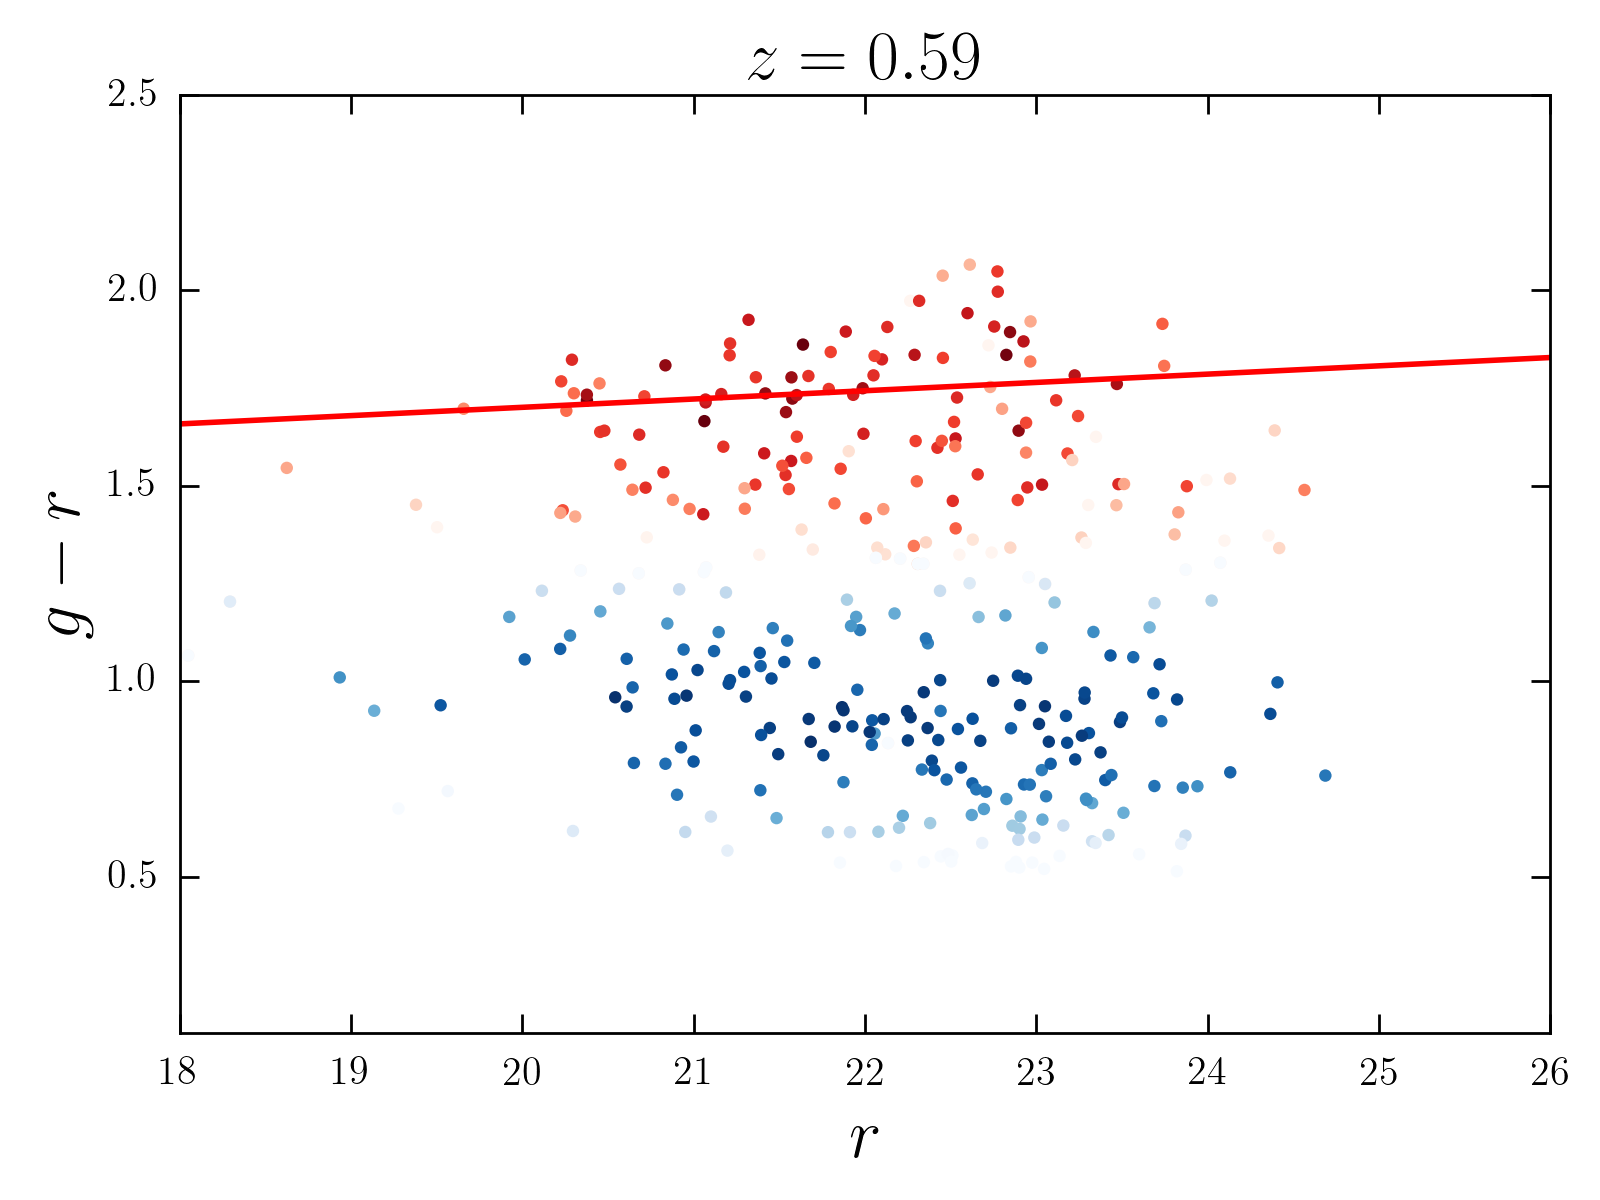
\includegraphics[width=0.7\textwidth]{./chapters/chapter6/figs/cl_test_rs.png}
\caption{Colour--magnitude diagram for a cluster at $z=0.59$ from the Y1 redMaPPer sample, given as an example (same as Figure \ref{fig:histcl}). The red points are weighted by $p_{\rm mem}\times p_{\rm red}$, and the blue points by $p_{\rm mem}\times p_{\rm blue}$ (where $p_{\rm blue}$ is defined similarly to the red sequence membership in Eq. (\ref{eq:prs})). The red line is the best fit from the GMM method.}\label{fig:slopecl}\end{figure}

\begin{figure}
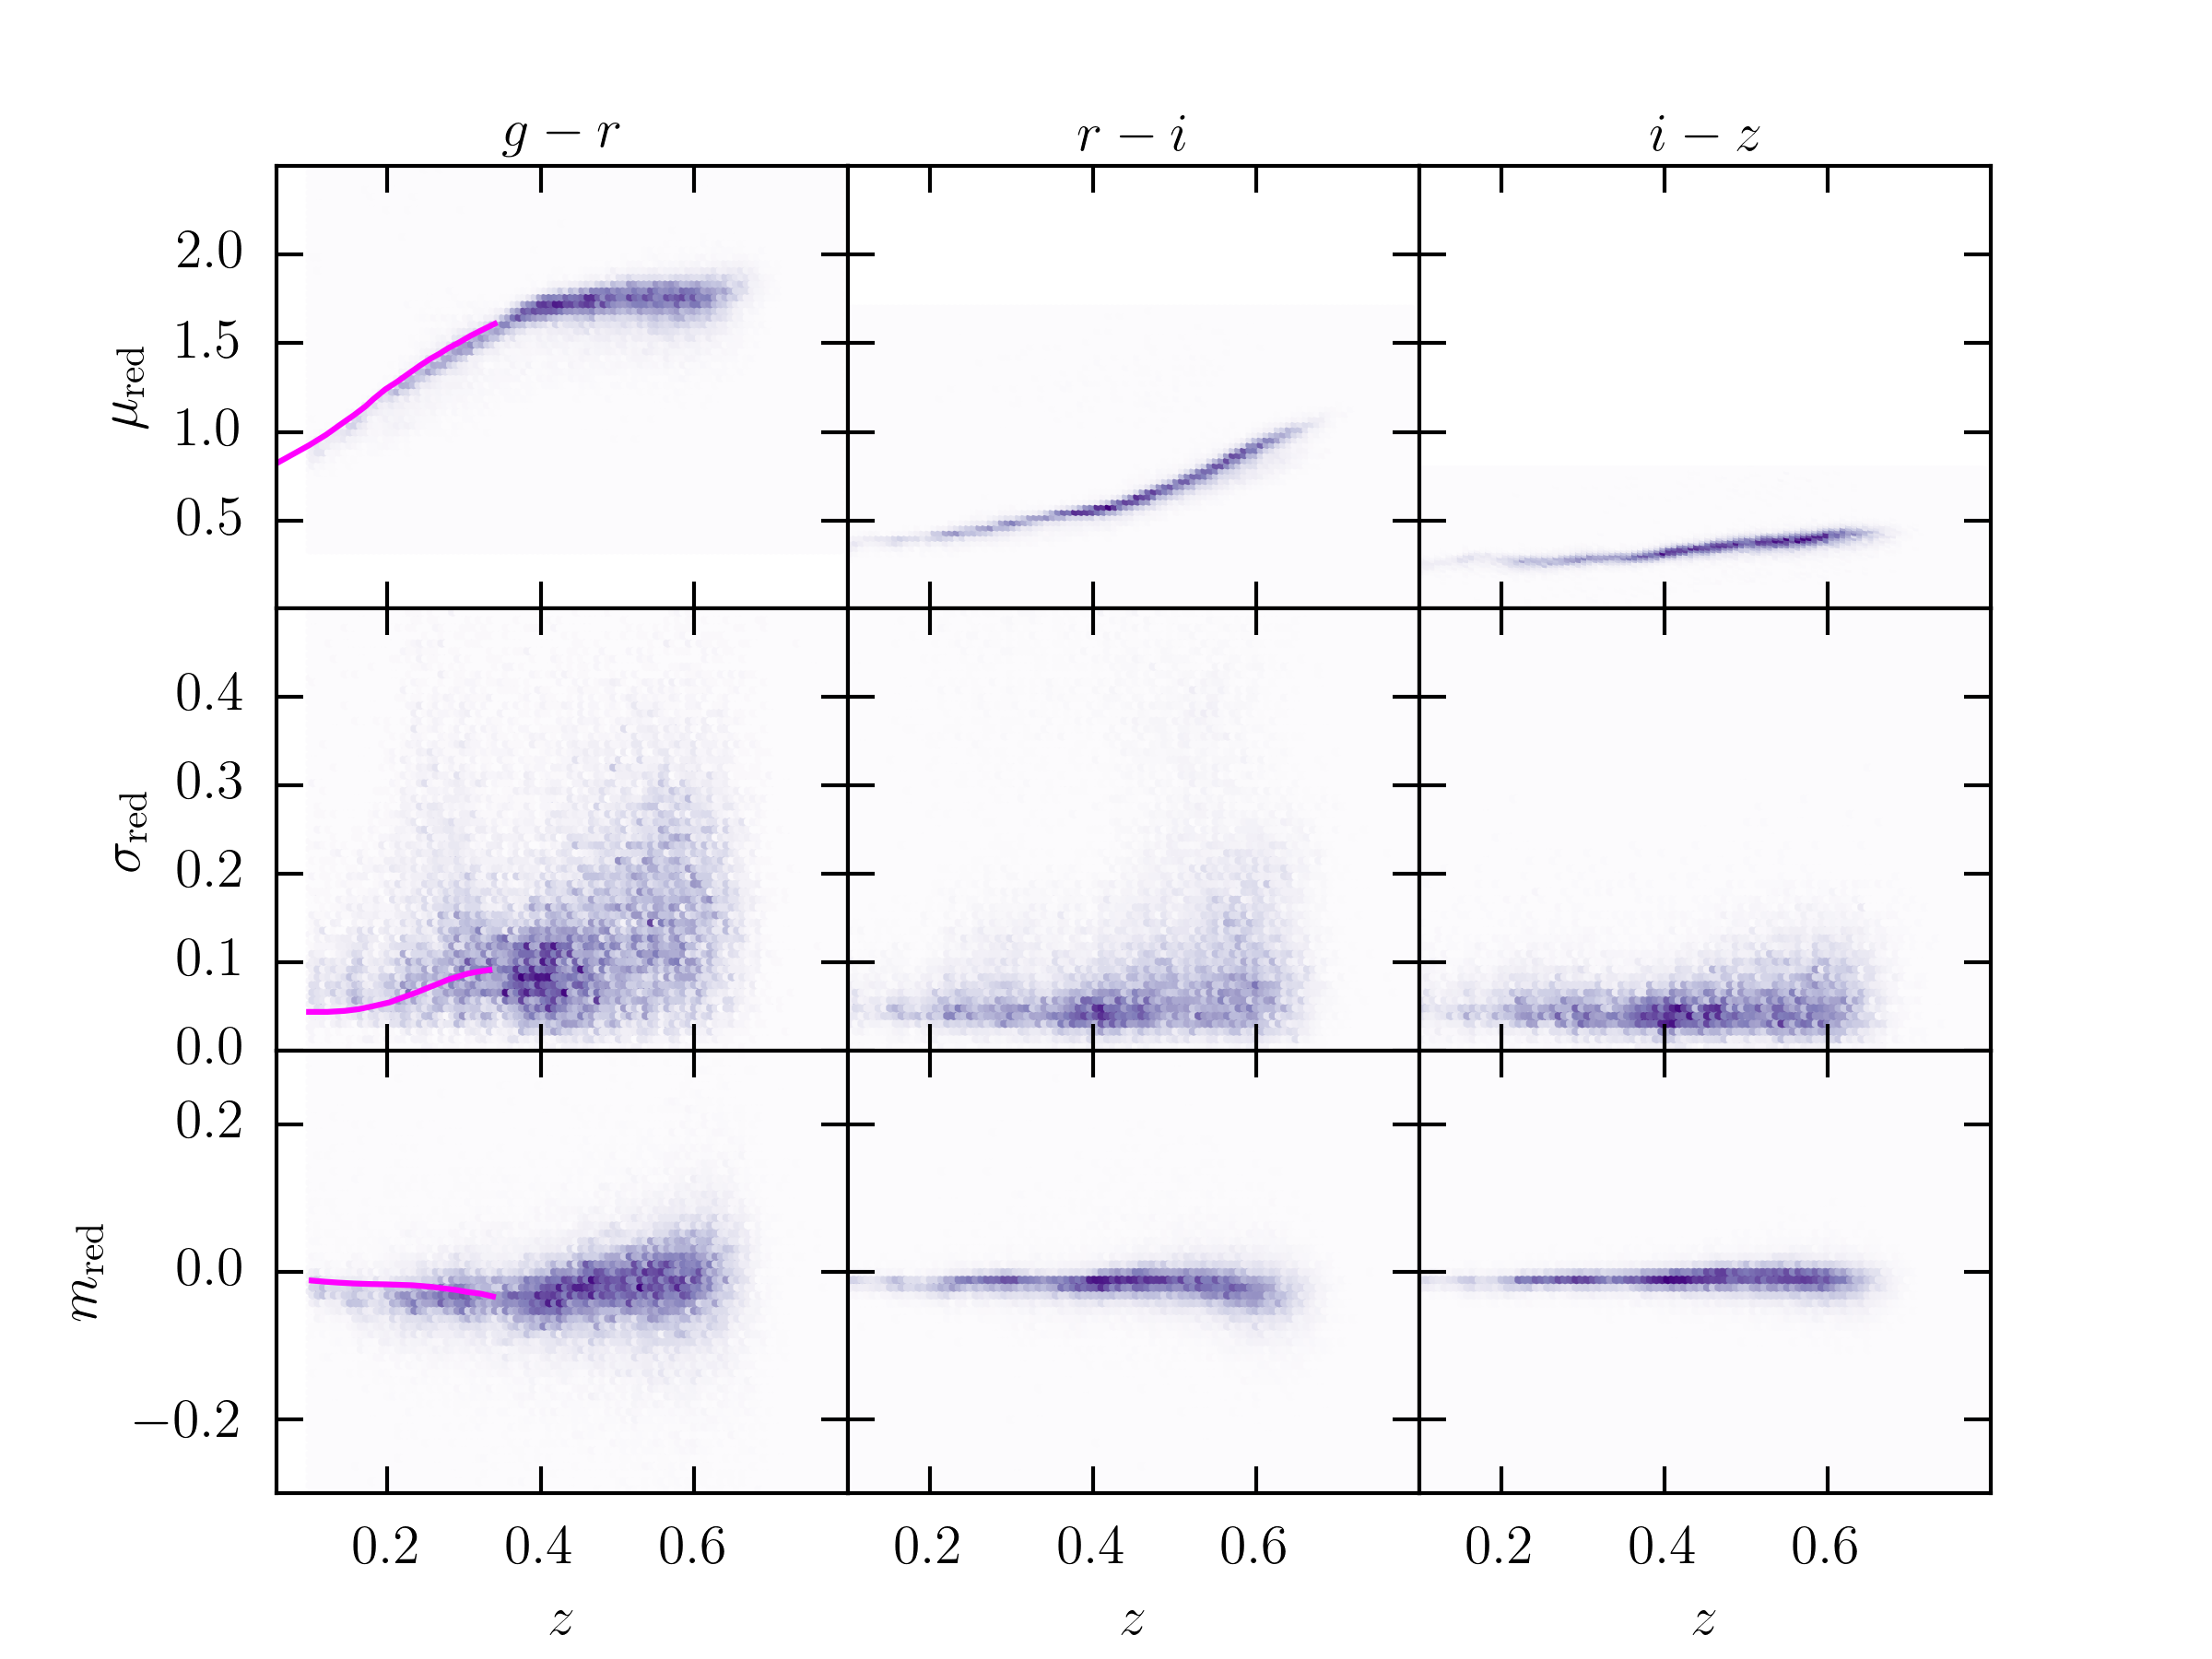
\includegraphics[width=1\textwidth]{./chapters/chapter6/figs/3x3_Mar18.png}
\caption{Red sequence mean colour $\mu_{\rm red}$, intrinsic scatter $\sigma_{\rm red}$ and slope $m_{\rm red}$ as a function of redshift for $\sim80,000$ clusters from the DES Y1 redMaPPer cosmology sample (purple density plot). The magenta lines are the estimates from redMaPPer using SDSS data (from \citealt{redpaper}), which are only volume limited out to $z\sim0.35$. These are shown for a qualitative comparison.}\label{fig:3x3}\end{figure}

Other quantities of interest in cluster studies are the mean colour and the scatter around it of the red sequence galaxies. These are measured by our GMM fit as the mean and the width of the Gaussian distribution associated with the red sequence. The observed scatter $\sigma_{\rm obs}$ will be given by the contribution of the intrinsic scatter in colour of the galaxies in the cluster and of the photometric error in the colour $\sigma_{\rm phot}$. Assuming these two errors are independent, they can be summed in quadrature, and the intrinsic scatter we are interested in is given by:
\begin{equation}
\sigma_{\rm int} =\sqrt{\sigma^2_{\rm obs}-\sigma^2_{\rm phot}}\,.
\end{equation}
The typical photometric error for each cluster can be measured as the mean measured colour error from its members. We consider only members with $p_{\rm mem}>20\%$ to avoid including a high number of interlopers. In Figure \ref{fig:3x3} we show red sequence mean colour $\mu_{\rm red}$, intrinsic scatter $\sigma_{\rm red}$ and slope $m_{\rm red}$ from the three considered colours as a function of redshift. These results can be compared to the results from \citet{redpaper} in $g-r$ for SDSS clusters. This comparison only consists in a qualitative check for our method, and is only valid out to $z=0.35$, which is the redshift out to which their sample is volume limited. The mean colours tend to become redder at higher redshifts, as expected. The intrinsic scatter increases, while also becoming a noisier measurements due to the fact that the photometric errors become more substantial, in particular in $g-r$, as most of these red sequence galaxies are very faint in $g$--band.  The fact that the intrinsic width of the red sequence increases with redshift, shows that red sequence--based cluster finders may face more difficulties in identifying clusters at higher $z$, and that including the blue cloud into mass proxies may be useful. The slope is negative and quite shallow, as seen in previous studies (e.g. \citealt{mei}, \citealt{redpaper}).
On--going work is focused on measuring the mentioned quantities, along with the blue fraction, from rest--frame galaxy colours. These measurements will allow physical interpretations of the evolution of the studied properties, which is not possible with the observed colours only. The results shown in Figure \ref{fig:3x3} for the observed colours still provide a solid consistency check for our membership probability assignment scheme. %The SDSS redMaPPer results are only shown for a qualitative comparison, given that the sample is shallower and incomplete at the higher redshifts we explore with DES, and that their definitions of colours and width are different.


\section{Stellar-to-halo mass}\label{shmrsec}
While the weak lensing calibration of the mass scaling relation for $\mu_\star$ is carried out in a companion paper for SDSS clusters (\citealt{maria}), here we use an independent mass estimate through the richness-mass relation which has been extensively studied for redMaPPer clusters in \citet{melchior}. This allows us to transform the redMaPPer richness $\lambda$ into a halo mass $M_{200m}$ for all the Y1 redMaPPer clusters and estimate the stellar--to--halo--mass relation for DES clusters. 

For the full Y1 redMaPPer sample we focus on a statistical measurement of the stellar to halo mass relation. This means that while binning our sample in halo mass and redshift, we assume that the intrinsic scatter of stellar mass around a certain halo mass would reduce to a stochastic scatter around the mean SHMR value. The validity of this assumption has already been pointed in other works (\citealt{zu}; \citealt{guo}). We therefore choose a method that allows us to fit an intrinsic scatter and to take into account errors on stellar mass, halo mass and redshifts.

We fit the SHMR with a linear model in ${\rm Log}(M_\star),~{\rm Log}(M_{200c}),~{\rm Log}(1+z)$ in the form:
\begin{equation}
{\rm Log}\Big(\frac{M_\star}{\tilde{M_\star}}\Big)=\alpha{\rm Log}\Big(\frac{M_{200c}}{\tilde{M}_{200c}}\Big)+\beta{\rm Log }\Big(\frac{1+z}{1+\tilde{z}}\Big)+\gamma~,\label{shmreq}
\end{equation}
where $\tilde{M}_\star$, ${\rm Log}(\tilde{M}_{200c})=13.79$ and $\tilde{z}=0.46$ are the median values of the full sample. $\tilde{M}_\star$ is changed from case to case. This empirical relation is a fair assumption at cluster scales, as also motivated by simulations, and it is often used in the literature (\citealt{brough}; \citealt{moster10}; \citealt{illustris}). We add a Gaussian scatter $\sigma_0$ on ${\rm Log}(M_\star/\tilde{M_\star})$ independent of halo mass, which enters in our analysis as an additional term to the covariance matrices of the data. We further assume that the measurements of the data $D_i$ for each cluster $i$, namely $M_{\star,i}$, $M_{200c,i}$ and $z_i$, are independent, and that the errors on the data are Gaussian. Under these assumptions, we calculate the posterior distribution of the parameters $\alpha,~\beta,~\gamma,~\sigma_0$ in Eq. (\ref{shmreq}) given the data $D$ for each cluster $i$:
\begin{multline}
p(\alpha,\beta,\gamma,\sigma_0|D)  = \prod_i p(\alpha,\beta,\gamma,\sigma_0|D_i)\\
\hspace{15pt}\propto  \prod_i \iiint  {\rm d} x_i ~{\rm d} y_i ~{\rm d} z'_i ~p(\alpha,\beta,\gamma,\sigma_0, x_i, y_i, z'_i|D_i)\\
\propto \prod_i\iiint {\rm d} x_i ~{\rm d} y_i ~{\rm d} z'_i ~ p(\alpha,\beta,\gamma,\sigma_0, x_i, y_i, z'_i) \times p(D_i | \alpha,\beta,\gamma,\sigma_0, x_i, y_i, z'_i)\,,
\end{multline}
where $x_i \equiv {\rm Log}\Big(\frac{M_{\star,i}}{\tilde{M_\star}}\Big)$, $y_i \equiv {\rm Log}\Big(\frac{M_{200c,i}}{\tilde{M}_{200c}}\Big)$, $z'_i \equiv {\rm Log }\Big(\frac{1+z_i}{1+\tilde{z}}\Big)$ and we have applied Bayes' theorem. Going forward: 
\begin{multline}
p(\alpha,\beta,\gamma,\sigma_0|D)  \propto \prod_i \iiint {\rm d} x_i ~{\rm d} y_i ~{\rm d} z'_i ~ p(x_i |\alpha,\beta,\gamma,\sigma_0, y_i, z'_i) p(\alpha,\beta,\gamma,\sigma_0, y_i, z'_i) \\
\times p(D_i | \alpha,\beta,\gamma,\sigma_0, x_i, y_i, z'_i)\,,
\end{multline}
where the first term is a 1D Gaussians $\mathcal{N}^{\rm 1D}(\mu;\sigma^2)$ of mean $\mu=x_i-\alpha y_i-\beta z'_i-\gamma$ and variance $\sigma_0^2$, and the last component is the likelihood of each cluster $i$, a 3D Gaussian in this case:
\begin{multline}
\hspace{-20pt}p(\alpha,\beta,\gamma,\sigma_0|D)  \propto \prod_i p(\alpha,\beta,\gamma,\sigma_0) \iiint {\rm d} x_i ~{\rm d} y_i ~{\rm d} z'_i ~ \mathcal{N}^{\rm 1D}(x_i-\alpha y_i-\beta z'_i-\gamma;\,\sigma_0^{2})\\
\hspace{7cm} \times \mathcal{N}^{\rm 3D}( [x_i-\bar{x_i};y_i - \bar{y_i}; z'_i - \bar{z}'_i];\,\Lambda) \\
\propto p(\alpha,\beta,\gamma,\sigma_0)  \prod_i \mathcal{N}^{\rm 1D}(\bar{x_i}-\alpha\bar{y_i}-\beta\bar{z}'_i-\gamma;\,\sigma_0^{2}+\Lambda_x+\alpha^2\Lambda_{y}+\beta^2\Lambda_{z'})\,, \label{eq:posterior}
\end{multline}
where $\Lambda$ is the covariance matrix of the $i-$th cluster, which is diagonal under our assumptions. We assume uniform truncated priors in $p(\alpha,\beta,\gamma,\sigma_0)$ for all of the four fitting parameters, in particular $0<\alpha<2$, $-2<\beta<2$, $-10<c<10$ and $0<\sigma_0<1$.

\begin{figure}\hspace{-2cm}
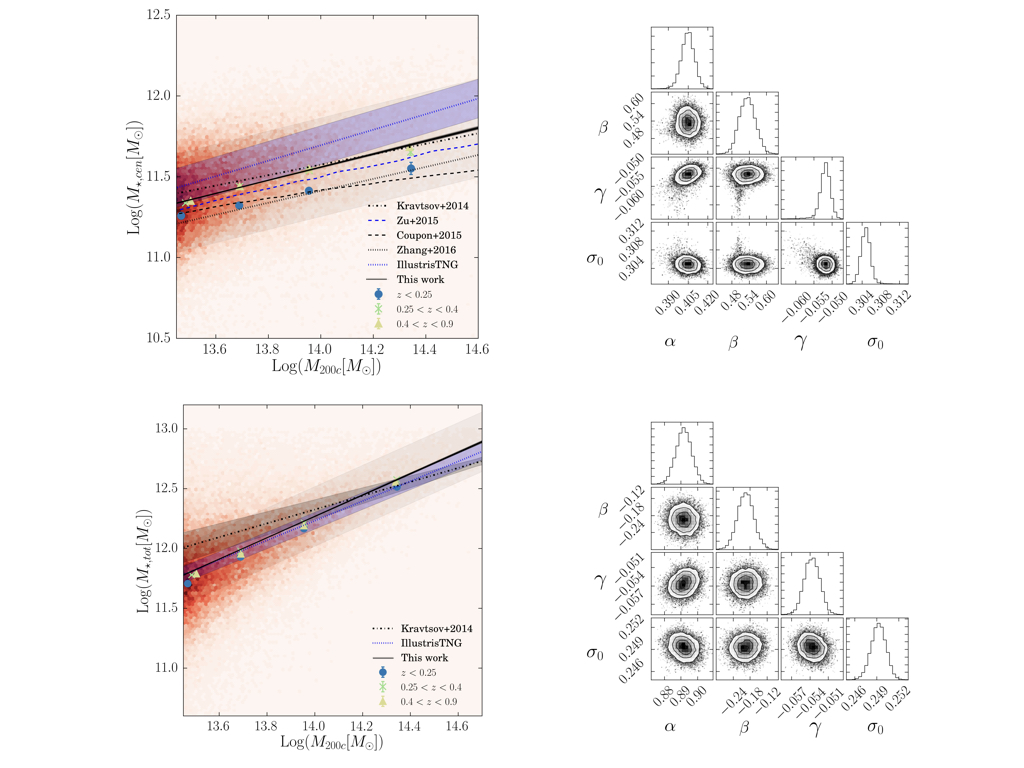
\includegraphics[width=1.3\textwidth]{./chapters/chapter6/figs/shmr_all_001.jpeg}
\caption{\emph{Top: }Stellar--to--halo mass relation for central galaxies (left panel), and posterior distributions of the parameters in Eq. (\ref{shmreq}) (right panel). \emph{Bottom: }Total stellar--to--halo mass relation (left panel), and posterior distributions of the parameters in Eq. (\ref{shmreq}) (right panel). The data points represent the mean stellar mass values and the standard error of the mean of the distribution in halo mass bins. Binned data are only shown to guide the eye, and have not been used in the analyses. The black lines are 100 random samples from our $\alpha$ and $\beta$ posterior distributions, and the light shaded broad region represents our scatter. The lines from the literature represent their best fit. The shaded region around the \citet{kravtsov} best fit is their 1$\sigma$ uncertainty on slope and intercept. The shaded region around the IllustrisTNG best fit is the \citet{illustris} scatter estimate for 32 kpc apertures around galaxies. All the data and fits presented assume a Chabrier IMF.}\label{shmrall}\end{figure}

\subsection{Central stellar mass to halo mass}

We select as the central the galaxy with highest $P_{\rm cen}$ centering probability from the redMaPPer catalog, and consider as satellites all of the remaining galaxies. We fit the stellar mass of centrals, $M_\star^{\rm cen}$, as a function of $M_{200c}$ and estimate the parameters in Eq. (\ref{shmreq}) and (\ref{eq:posterior}). The results are presented in Table \ref{fitstable} (where we report the median of the posterior distribution and 68\% confidence level uncertainties) and Figure \ref{shmrall}. The scatter at fixed halo mass is substantial ($\sim 0.3$ in logarithmic scale) but a trend with halo mass is clearly found, with a slope of $\alpha=0.4052\pm 0.0048$. 
In Figure \ref{shmrall} we show the results for redMaPPer clusters in the red density plot, while the black solid lines are 100 random samples from the $\alpha$ and $\beta$ posterior distributions obtained with the Bayesian linear regression on that data. For visualisation purposes, we plot mean stellar mass values in halo mass bins in three redshift bins ($z<0.25$, $0.25<z<0.4$, $0.4<z<0.7$). These results are compared to others from the literature that use a range of different methods. For a more consistent comparison, we show results that assume a Chabrier IMF. \citet{kravtsov} use SDSS photometry and X-ray data for single clusters at $z<0.1$ and compare with abundance matching predictions, while \citet{zu} and \citet{coupon} implement HOD methods on SDSS and CFHTLS data respectively. \citet{zhangbcg} present a study of BCGs from DES Science Verification data for X-ray selected clusters, and we show their results for 32 kpc apertures around the BCG at the mean redshift of our sample $z=0.45$. \citet{illustris} use the latest Illustris simulations to measure the stellar mass content of groups and clusters.

\citet{kravtsov} perform a detailed analysis to derive extended luminosity profiles around BCGs, and fit those with multiple S\'ersic profiles. The model profile is then extrapolated to infinity to derive total magnitudes. They find that \texttt{CMODEL} magnitudes computed with the standard SDSS pipeline underestimate the total BCG luminosity by a factor $\sim 2-4$. The MOF magnitudes used in this work are computed similarly to the SDSS \texttt{CMODEL} magnitudes: a composite model made of a bulge plus a disk component is fit to the profile and extrapolated to infinity. In order to compare our results to \citet{kravtsov} we downweight their best fit by 0.45 dex in stellar mass. This is their SHMR estimate presented in Figure \ref{shmrall}, which is consistent with our result  at all halo masses, but with a slightly shallower slope. They find a slope of $0.39\pm0.17$ and $0.33\pm0.11$ when they include the clusters from \citet{gonzalez} (and this is the result we show), which is within 1$\sigma$ from our best--fit. The de--corrected normalisation is consistent with ours, although they focus on clusters at $z<0.1$ and our data points from the lowest redshift bin are $\sim 0.1$ dex below the rest of the cluster sample. This discrepancy is comparable to the uncertainty on stellar masses and could be due to the difference in the photometry and the qualitative correction we have applied. %at low halo masses ($M_{200c} \lesssim 10^{14} M_\odot$). At higher masses and luminosities, where the SDSS standard magnitudes are expected to more significantly underestimate the true luminosity of the galaxies, we believe that the MOF method is performing better than \texttt{CMODEL} magnitudes.

The analysis from \citet{zu} is also valid at low redshifts ($z<0.3$) and it looks qualitatively in agreement with our lowest redshift bins measurements. The slope from \citet{icl} of $0.37\pm 0.10$ is within $1\sigma$ of what we find, while the normalisation depends on the aperture chosen and a comparison is not straightforward: we use magnitudes from MOF, that are not computed within a fixed aperture but vary from object to object. 
%is shallower than ours, but they find different results at different halo masses, which they report as a possible consequence of the temperature--to--halo--mass relation dependence on halo mass.

The \citet{coupon} estimate has the shallowest slope of all the results discussed here, which makes their results deviate from ours towards halo masses. Their redshift range is overlapping with ours from $z>0.5$, but going up to $z\sim 1$ with a mean around 0.8. It is possible that galaxy evolution affects the stellar mass of galaxies at redshifts that we are considering in this work, but the weak redshift evolution that we observe seems to go towards higher values of stellar mass at higher $z$. We argue that the difference in normalization may be due to the different framework used to estimate the stellar masses. In particular, they utilize a wider range of galaxy dust models, which they may constrain better thanks to the $K_s$ band information. Also, they do not consider models with supersolar metallicity, which may be relevant when fitting BCGs and luminous red galaxies in clusters. 

Results from the latest IllustrisTNG simulations (\citealt{illustris}) deviate from our result and other observational data at high halo mass. In Figure \ref{shmrall} we plot their best fit SHMR for centrals when the stellar mass is computed within a 30 kpc aperture. They de-correct \citet{kravtsov} result to match that aperture and find their best fit to be higher than \citet{kravtsov}. They find that the SHMR is very sensitive to the change of aperture considered, which could also explain our disagreement. In particular, for brighter (and thus greater stellar mass) objects we may be systematically underestimating the total luminosity of the central galaxy (as also pointed in \citealt{kravtsov}), as we are only considering a model that fits well to the inner luminosity profile, and not the extended stellar halo. Also, in brighter environments, there is a chance that the subtracted background is overestimated. This would explain our shallower slope in the SHMR. On the other hand, we find a high scatter ($\sim 0.3$ dex) in stellar mass that still makes our results consistent at the high mass end.

Our scatter is larger than typically found in other works (0.22 dex in \citealt{zu} and \citealt{coupon}, 0.17 dex in \citealt{kravtsov}). Uncertainties on the photometry, stellar masses, total masses and so on can well affect the value of the intrinsic scatter. Given the differences between the methods and samples adopted, we believe that it is reasonable to find different values. However, our sample spans a wider combination of area and redshift range than other works, making contributions to the intrinsic scatter from sample variance and galaxy or cluster evolution more substantial. Amongst the works discussed in this section, the analysis from \citet{kravtsov} is the closest to ours. They consider a much smaller ($\sim$ tens of clusters) sample of clusters over a redshift range $z<0.1$, thus it is not surprising that our scatter is $\sim 0.12$ dex larger than theirs. 

The redshift dependence of the SHMR seen in the $\beta$ parameter is positive, and this can be understood in light of the results presented in Section \ref{sec:cengrowth}.

\begin{figure}\centering 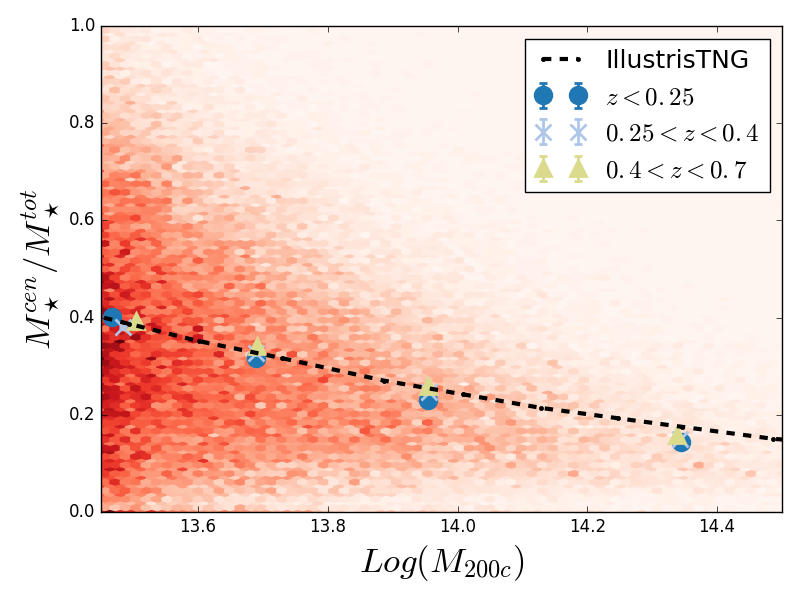
\includegraphics[width=0.7\textwidth]{./chapters/chapter6/figs/fcen_chab_Dec17.png}\caption{Stellar mass of the central over the total stellar mass for the Y1 redMaPPer clusters (red density plot). The data points represent the median stellar mass fraction values at different halo masses and the errorbars indicate the standard error of the mean of the fraction distribution in each halo mass bin. The central contributes roughly 40-20\% of the total stellar mass. The line is from \citet{illustris} results at $z=0$ and with 30 kpc apertures.}\label{smcentot}\end{figure}

%%%%Maybe add this paragraph in the Intro
%As shown in previous works (e.g. \citealt{zu}) the star formation efficiency peaks at Milky way-like masses ($\sim 10^{12} h^{-1} M_\odot$) and drops in halos above that mass. This is usually explained with AGN feedback in high mass halos (e.g. \citealt{agn}), but observational constraints have not quite reached a consensus on this efficiency, rendering it hard to constrain also feedback processes.

\begin{sidewaystable} % <-- HERE
\centering
\begin{tabular}{c|cccccc}
IMF &$$&$\alpha$&$\beta$&$\gamma$& $\sigma_0$ & ${\rm Log}(\tilde{M_\star})$\\
\hline
Chabrier & Central & $0.4052^{+0.0048}_{-0.0048}$ & $0.531^{+0.030}_{-0.030}$ & $-0.0520^{+0.0013}_{-0.0014}$ & $0.3048^{+0.0009}_{-0.0010}$& 11.52\\
& Satellites & $1.1351^{+0.0063}_{-0.0066}$ & $-0.332^{+0.037}_{-0.037}$ & $-0.1285^{+0.0016}_{-0.0016}$ & $0.2512^{+0.0013}_{-0.0013}$& 12.01\\
& Total & $0.8918^{+0.0048}_{-0.0048}$ & $-0.194^{+0.028}_{-0.028}$&$-0.0536^{+0.0012}_{-0.0013}$&$0.2492^{+0.0010}_{-0.0010}$ & 12.12 \\
\hline
Salpeter & Central & $0.4042^{+0.0050}_{-0.0054}$ & $0.642^{+0.032}_{-0.042}$ & $-0.0549^{+0.0012}_{-0.0013}$ & $0.30216^{+0.00099}_{-0.00094}$& 11.56\\
& Satellites & $1.1181^{+0.0065}_{-0.0067}$ & $-0.2863^{+0.037}_{-0.035}$ & $-0.1010^{+0.0016}_{-0.0016}$ & $0.2368^{+0.0014}_{-0.0014}$& 12.22\\
& Total & $0.8653^{+0.0053}_{-0.0050}$ & $-0.116^{+0.028}_{-0.032}$&$-0.0401^{+0.0012}_{-0.0012}$&$0.2320^{+0.0010}_{-0.0010}$ & 12.28 \\
%\hline
%Salpeter & Central & $0.3882^{+0.0043}_{-0.0045}$ & $0.652^{+0.028}_{-0.027}$ & $-0.0510^{+0.0012}_{-0.0011}$ & $0.33083^{+0.00095}_{-0.00088}$ & 11.79\\
%& Satellites & & &\\
%& Total & $0.9984^{+0.0043}_{-0.0043}$ & $1.1216^{+0.029}_{-0.032}$&$-0.0631^{+0.0012}_{-0.0012}$&$0.3972^{+0.0011}_{-0.0011}$ & 12.55\\
\end{tabular}\caption{Fits of the SHMR from Eq. (\ref{shmreq}) 
for centrals and all galaxies.  Values represent the median of the parameters posterior distribution, and the errors are at 68\% confidence level. Redshift and halo mass pivot values are respectively $\tilde{z}=0.46$ and ${\rm Log}(\tilde{M}_{200c})=13.79$.}\label{fitstable}

\end{sidewaystable} % <-- HERE


%\begin{table*}\centering
%\end{table*}

\begin{figure}\centering
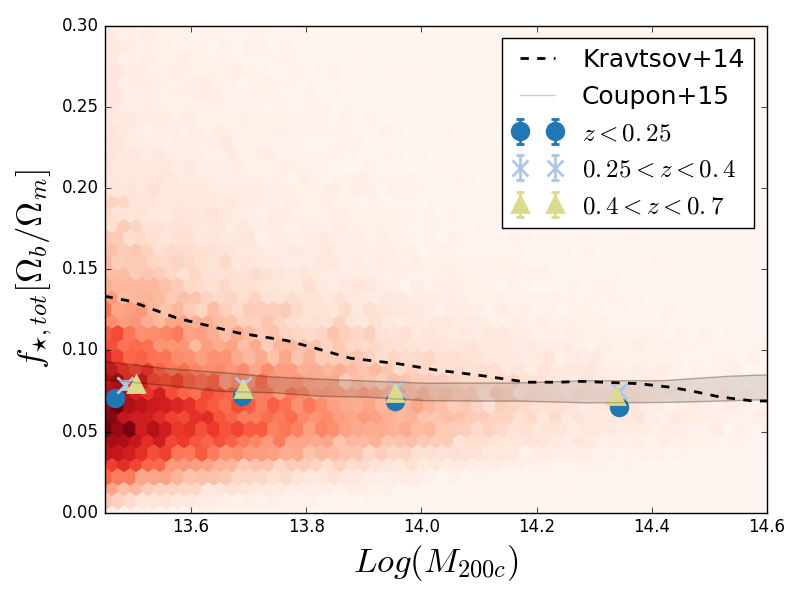
\includegraphics[width=0.7\textwidth]{./chapters/chapter6/figs/f_star_tot_chab_Dec17.png}
\caption{Stellar mass fraction (total stellar mass of each cluster over its halo mass) as a function of halo mass. The data points represent the mean stellar mass fraction values at different halo masses and the error bars indicate the standard error of the mean. The dashed line is the prediction of \citet{kravtsov} using abundance matching with scatter in the SHMR and a Chabrier IMF. The stellar masses have been corrected to galaxies within $R_{200c}$ only for the comparison.}\label{fstot}\end{figure}

\subsection{Total stellar to halo mass}\label{SHMRtot}

Satellite galaxies become a significant contribution to the stellar content of the halo at higher halo masses. In fact, the total mass of clusters can be accounted for by the contribution of the satellite sub-halos, while the central halo contribution decreases. This can be seen in terms of stellar mass in Figure \ref{smcentot}. The central contributes roughly 40-20\% of the total stellar mass at all halo masses, decreasing with halo mass. We do not find any significant redshift dependence of this behavior, but we recover a significant scatter at lower masses (as also found in \citealt{illustris}, where it is $\lesssim 0.2$ dex below ${\rm Log}(M_{200c})\sim 14$).

Fit results for the total SHMR with the power law presented in Eq. (\ref{shmreq}) are listed in Table \ref{fitstable} and shown in Figure \ref{shmrall}. Our errors on the power law parameters are very small, in the order of $\sim 0.5-7 \%$, because of the large number statistics used. We find that the total SHMR follows a steeper and less scattered power law than centrals only, as also found in previous works (e.g. \citealt{illustris}). 
The slope is significantly steeper than what is found in other observational works, such as \citet{andreon12} $0.37\pm0.07$, and \citet{kravtsov} $0.59\pm 0.08$, while the central SHMR slope is still consistent with \citet{kravtsov} within 1$\sigma$. One reason for the discrepancy is that they consider a fixed $M_\star/L$ ratio to compute the stellar masses of all galaxies. Secondly, we have a deeper dataset and MOF photometry that performs well in crowded environments such as clusters, and membership probabilities that take into account the galaxy properties. These factors will change the contribution that the satellite galaxies give to the total stellar mass of clusters. Our result is closer to what is found in the latest IllustrisTNG simulations: $0.84$ when including centrals, intra--cluster light (ICL) and satellites, reaching $1.14$ for satellites only. This value is also less than 1$\sigma$ away from our result. The inclusion of centrals is what lowers the slope, an effect which is mitigated in our case by the inclusion of membership probabilities, given that we do not have a truth table of members. In fact, centrals will also have $p_{\rm mem}<1$ by construction.

Our analysis shows that the total SHMR has a weaker dependence on redshift than for centrals, with the value of $\beta$ being closer to 0. However the inversion in sign of $\beta$ is due to the probabilities that are used to weight the stellar masses, and this is an unavoidable effect due to our survey specifics. In fact, the stellar mass of the redshift bin containing galaxies around $z\sim 0.4$ is larger than the others. The number density of DES galaxies shows in fact a peak around that redshift: more galaxies are assigned to a similar photo-$z$ there compared to other redshifts, and therefore they will have a larger contribution from the $p_{z}$ component in the membership probabilities. At the same time more constraining power will come from the higher redshifts with lower stellar masses, because there are more clusters there in our volume limited sample. We therefore believe that the observed redshift dependence of the total SHMR is mostly due to the photometric redshifts rather than to any physical evolution.

%At the same time, we have to take into account two factors: 1. clusters that have a certain halo mass today, have lower mass progenitors at higher redhsifts, 2. heterogeneous cluster samples have been used in many works to  estimate the SHMR. {\bf what is the conclusion of this paragraph?}

The amount of scatter in stellar mass at fixed halo mass is also an important ingredient for halo or sub-halo abundance matching (AM) methods, and \citet{kravtsov} showed how the scatter can impact the SHMR measurements. Our 1-$\sigma$ scatter in the logarithmic stellar mass at fixed halo mass is $0.2492\pm 0.0010$. For AM a scatter of $\sim 0.1-0.3$ is usually assumed.
The intrinsic scatter found in the other works discussed here (e.g. \citealt{illustris}, \citealt{leauthaud} and \citealt{kravtsov}) is usually $0.1-0.25$ dex. As discussed for the centrals, we believe that the difference in scatter is due to the different samples and methods used. We note that our result is consistent with the analysis by \citealt{leauthaud} ($\sim 0.2-0.25$ dex over $0<z<1$), who performed a joint analysis of galaxy--galaxy weak lensing, galaxy spatial clustering, and galaxy number densities with COSMOS data. We refer to future work to introduce a redshift and halo mass dependent intrinsic scatter.

We find a scatter in halo mass at fixed stellar mass of $\sigma_{{\rm Log}(M_{200c})|M_\star}\sim 0.17$. Our result is similar to what \citet{andreon12} finds for the scatter at fixed stellar mass (0.21-0.32 dex). This value can also be compared to what we find in the halo mass--$\mu_\star$ from the X-ray temperature calibration, $\sim 0.18$, and they are very close despite the fact that they have been derived very differently.
%\citealt{chiu17} find a higher scatter in the SHMR compared to the ICM-to-halo relation, with the ICM being estimated from X-ray \emph{Chandra} data. This is a motivation to think that the higher scatter we find in $T_X$ is at least partially intrinsically due to the physical interplay between the X-ray emitting matter and the total cluster mass, and between the stellar mass and the total mass. 
However, to truly compare the scatter on a physical level, one would need to understand the correlation between the parameters and the selection effects introduced by the X-ray selection. Even though the X-ray measurements are done at the redMaPPer cluster positions, a cut in the temperature SNR is essential to avoid taking into account spurious detections. This selection introduces a redshift and mass dependent cut on the sample (a Malmquist bias). 

We find that the total stellar mass fraction $f_\star=M_\star^{tot}/M_{200c}$ is $\sim 0.011$, and it is flat over the range of halo masses studied. The results are shown in Figure \ref{fstot}, where we normalize by the baryon-to-matter mass ratio from cosmological constraints $\Omega_b/\Omega_m \simeq 0.16$ (\citealt{planck16}) for a better understanding of the fraction of baryons locked into stars: roughly $7\%$ of cluster baryons are transformed into stars. The stellar masses have been corrected to galaxies within $R_{200c}$ for the comparison, as our analysis brings the total stellar mass of clusters out to 3 Mpc (although contributions outside $\sim 1.5$ Mpc are negligible because of the radial membership probabilities), which is roughly $30\%$ higher than the mass within 1 Mpc. The radial probability gives most of the weight to the galaxies within $R_{200c}$, and extensive studies have been performed on mock data so that $\Sigma p_{mem}\sim N_{\rm members}$. We therefore believe that our total stellar mass is a good estimator of the whole cluster stellar mass besides the ICL.

Despite some possible difference in the stellar mass measurements that could be due to the mass-to-light ratio assumed, of the different cluster selection, our results confirm what is found in \citet{kravtsov}: the suppression of star formation efficiency at larger halo masses is not as  strong as previously expected (e.g. \citealt{behroozi}), and that is due to the contribution of satellites that makes this efficiency a milder function of halo mass compared to centrals alone. Also \citet{illustris} find that the $f_\star$ dependence on halo mass is shallower at the high mass end, dropping only by a factor of $\sim 2$ with respect to Milky Way halo masses. 
\citet{coupon} find that the total stellar mass fraction is close to flat at cluster scales, slightly increasing at the high mass end. %Their result lies below our mean values, although their work is valid at $0.5<z<1$, where one might expect the stellar mass fraction to be lower (\citealt{illustris}, although there have been contrasting results, e.g. \citealt{leauthaud}).
A roughly flat stellar mass fraction at cluster masses is also explained in \citet{leauthaud}, who find once again results close to ours. They claim that flatness is due to galaxy merging in the absence of significant star formation. Above the peak in $f_\star$ at Milky Way halo masses, halos can only grow because of merging with halos of lower stellar mass fraction, therefore lowering the total $f_\star$. Towards higher halo masses, this means that the stellar mass fraction will be enhanced by the mergers, inverting the trend again. This behaviour will repeat towards increasing halo masses, causing the flattering.
%A stellar mass fraction value of 1\% is consistent with the asymptotic value found in other observational studies that also stack stellar mass fraction profiles, as in \citet{bahcall}, and in abundance matching analyses such as \citet{coupon}.

As for the total SHMR, we do not find evidence of redshift evolution in the stellar mass fraction. \citet{chiu16} and \citet{chiu17} also find that the stellar mass fraction in X-ray and SZ selected clusters depends only weakly on redshift, implying that the stellar content at a given halo mass changes very little since $z\sim 0.7$. Similar results are found in simulations, as in \citet{illustris}: the overall cluster stellar mass build-up happens at a similar pace as the dark matter halo assembly, resulting in very little change from redshift 1. \citet{chiu17} also point out that in the hierarchical formation scenario, this means that at these redshifts the halos mainly accrete from structures outside the virialised halo that have a stellar mass fraction close to the cosmic mean. 

Previous works found no or little dependence (\citealt{vulcani}; \citealt{etherington}) of the faint end galaxy stellar mass function on environment. We choose to employ the SMF from \citet{capozzi}, that was estimated for the whole DES SV COMMODORE galaxy catalog. They use a double Schechter function \citep{Schechter} the lowest redshift bin ($z<0.2$), and a single Schechter function in the higher bins. By integrating the GSMF best fits, we find that our total stellar mass would be $23-24\%$ higher if we were to include all galaxies below the $10^{10}M_\odot$ limit chosen, although this would have to be weighted by the membership probabilities for consistency.

In \citet{icl} we find that the central plus ICL contribution in low redshift ($0.2<z<0.3$) Y1 redMaPPer clusters is $\sim 40\%$ of the total stellar mass computed as in this paper, meaning that the ICL contribution to the total stellar mass can be up to $\sim 30\%$, bringing the stellar mass fraction up by a factor up to 1.3. Note that this factor would include also the contribution coming from undetected members, so it would at least partially take into account the low mass end of the SMF mentioned in the previous paragraph.


%%%%%%%%%%%%%%%%% EVOLUTION OF CLUSTERS PROPERTIES %%%%%%%%%%%%%%

\section{Stellar mass functions}\label{sec:smf}

\begin{table*}\centering
\begin{center}\textsc{Centrals}\end{center}
\begin{tabular}{c|cccc}
\hline
\hline
IMF &&$A\, {\rm [Mpc^{-3}]}$&${\rm Log} M_{\star,c}$&$\sigma_c$\\ %&$\chi^2_{\rm red}$\\
\hline
Chabrier &$\langle z \rangle \sim 0.2$ & $(5.791 \pm 0.098)\times 10^{-4}$&$11.4131 \pm0.0044$ & $0.2487\pm 0.0032$\\ % & 2.1\\
& $\langle z \rangle \sim 0.4$ & $(4.876 \pm 0.083)\times 10^{-4}$ &$11.481\pm 0.0043 $ &  $0.2425 \pm 0.0027$\\ % & 2.5\\
& $\langle z \rangle \sim 0.6$  &$(3.042 \pm0.038)\times 10^{-4}$& $11.462\pm 0.0031 $ &  $0.2417  \pm 0.0022 $  \\%& 3.0 \\
& Whole  &$(4.828 \pm0.037)\times 10^{-4}$& $11.461\pm 0.0019 $ &  $0.2455  \pm 0.0014^{\rm stat} $ \\% & 3.1 \\
&&&&$\pm 0.05^{\rm syst}$\\

\hline
Salpeter &$\langle z \rangle \sim 0.2$ & $(8.67 \pm 0.016)\times 10^{-4}$&$11.6687 \pm 0.0049$ & $0.2515\pm 0.0036$  \\%&3.9\\
& $\langle z \rangle \sim 0.4$ & $(7.33 \pm0.10)\times 10^{-4}$ &$11.744\pm 0.0036 $ &  $0.2485 \pm 0.0027$ \\%&5.0\\
& $\langle z \rangle \sim 0.6$ & $(4.54 \pm0.69)\times 10^{-4}$ &$11.728\pm 0.0039 $ &  $0.2421 \pm 0.0028$ \\%& 5.5\\
& Whole  &$(7.249 \pm 0.074)\times 10^{-4}$& $11.7251\pm 0.0026 $ &  $0.2478  \pm 0.0020 $\\%& 5.3 \\
\end{tabular}
\vspace{0.1cm}
\begin{center}\textsc{Total}\end{center}
\begin{tabular}{c|cccc}
\hline
\hline
IMF &&$\phi^*\, {\rm [Mpc^{-3}]}$&${\rm Log} M^*$&$\alpha$\\ %&$\chi^2_{\rm red}$\\
\hline
Chabrier &$\langle z \rangle \sim 0.2$ & $(1.68 \pm 0.16)\times 10^{-4}$&$11.510 \pm 0.026$ & $-1.267\pm 0.0038$\\% & 0.21\\
& $\langle z \rangle \sim 0.4$ & $(1.841 \pm 0.088)\times 10^{-4}$ &$11.460\pm 0.013 $ &  $-1.185 \pm 0.022$\\% & 0.08\\
& $\langle z \rangle \sim 0.6$ & $(1.228 \pm 0.083) \times 10^{-4}$ &$11.395\pm 0.019 $ &  $-1.108 \pm 0.034$\\% & 0.31\\
& Whole & $(2.02 \pm 0.11) \times 10^{-4}$ &$11.401\pm 0.019 $ &  $-1.119 \pm 0.025$\\% & 0.31\\
%& Whole  &$(6.287 \pm0.071)\times 10^{-5}$& $11.459\pm 0.0028 $ &  $0.1961  \pm 0.0020 $& 2.3 \\
\hline
Salpeter &$\langle z \rangle \sim 0.2$ & $(2.009 \pm 0.036)\times 10^{-4}$&$11.713 \pm 0.057$ & $-1.1845\pm 0.0066$\\% & 0.66\\
& $\langle z \rangle \sim 0.4$ & $(2.28 \pm 0.15)\times 10^{-4}$ &$11.659\pm 0.022 $ &  $-1.074 \pm 0.028$\\% & 0.15\\
& $\langle z \rangle \sim 0.6$ & $(1.57 \pm 0.16) \times 10^{-4}$ &$11.574\pm 0.035 $ &  $-0.955 \pm 0.051$ \\% & 0.68\\
& Whole & $(2.47 \pm 0.20) \times 10^{-4}$ &$11.593\pm 0.032 $ &  $-1.010 \pm 0.035$\\% & 0.31\\

\end{tabular}

\caption{Best--fit results of the SMF for centrals and all galaxies in the clusters in redshift bins and for the whole redMaPPer catalog. The redshifts reported are the mean values. The parameters are presented in Eq. (\ref{eq:smf}) and Eq.(\ref{eq:smf_tot}). Fits are performed over the stellar mass range (${\rm Log}(M_{\rm cen}/M_\odot)$) between 10.5 (10.3) and 12.5 for the centrals (total) SMF. These values are 0.2 dex higher for the Salpeter IMF case. }\label{tab:smf}
\end{table*}


\subsection{Central stellar mass function}

Several works (e.g. \citealt{lauer}) find that the luminosity function of BCGs follows a log-normal distribution. Given that we expect a similar $M_\star/L$ for these galaxies, it is reasonable to expect that also the SMF of centrals follows a similar behaviour, as also found in \citet{yang} for SDSS galaxy groups. In order to compute the SMF, we divide the stellar mass distribution by the comoving volume over the Year 1 footprint and by the bin width in stellar mass (0.15 dex). We estimate errors by making 200 bootstrap resamplings. Given the huge size of the cluster sample used, these errors are 2-3 orders of magnitude smaller than the SMF values. In Figure \ref{fig:smf} we show our results from a least--$\chi^2$ fit in redshift bins for a log--normal function in the form:
\begin{equation}
\phi_{\rm cen} (M_\star)=\frac{A}{\sqrt{2\pi}\sigma_c}\exp{\Big[ -\frac{({\rm Log} M_\star-{\rm Log} M_{\star,c})^2}{2\sigma_c^2} \Big]}\,,\label{eq:smf}
\end{equation}
where ${\rm Log}M_{\star,c}$ is by definition the expectation value for the logarithm of the stellar mass of centrals and $\sigma_c = \sigma({\rm Log}M_\star)$. The SMF for the whole redshift range has been computed by dividing by the ``effective'' comoving volume of the redMaPPer catalog: it takes into account the masking and depth variations over the footprint. The best--fit parameters for the two redshift bins and the whole sample are presented in Table \ref{tab:smf}. We also find that the mass function has a similar behavior when binning in halo mass [i.e. the conditional luminosity function $\phi_{\rm cen} (M_\star|M_{200c})$]. 

In order to estimate the systematic contribution to the SMF from the photometry and stellar model selection, we assume the errors on the stellar masses to be Gaussian and randomly draw 200 ``noisy'' stellar mass values $M_\star^{\rm noise}$ for each galaxy. The Gaussian width is given by the error estimate from the BMA code, as this will reflect the stellar population model uncertainty, as well as the photometry errors. The 16th and 84th percentiles of the SMF from such resampling are shown in the grey region in Figure \ref{fig:smf}. As we could have expected, this resampling has the effect of broadening the distribution (shown by the black points) because the uncertainty on the stellar masses has the effect of scattering the galaxies within different bins. This effect is known as the Eddington bias. Given that we assume the resampled stellar mass distribution to be a Gaussian in the logarithm of the stellar mass (as done also in \citealt{caputi}) convolved with the SMF which is also Gaussian, the result is that the measured SMF has the Gaussian widths added in quadrature. The width of the ${\rm Log}(M^i_\star)-{\rm Log}(M_\star^{i,{\rm noise}})$ distribution is 0.05 and we consider this effect as a systematic error from the photometry on the width $\sigma_c$.

The systematic error on $M_{\star,c}$ is driven by the IMF choice (see Section \ref{sec:imf}). The results are reported in Table \ref{tab:smf}. The reduced $\chi^2$ are high because of the contribution coming from the low mass end (${\rm Log}M_\star\lesssim 10.8$): the SMF is not log--normal there. Assuming the abundance matching theory, where the central stellar mass function at fixed halo mass has a log--normal scatter in $M_\star$, then the convolution of those distributions would be Gaussian in ${\rm Log} M_\star$ over the clusters halo mass range. We tested this using the Buzzard simulations (\citealt{derose}; \citealt{wechsler}) made for DES Year 1 data: when the true centrals for halo masses $M_{200c}>10^{13} M_\odot h^{-1}$ are selected, no deviation from Gaussianity is seen in the luminosity function (LF) in absolute magnitude space (see Figure \ref{fig:smfbuzzard}). On the contrary, when redMaPPer centrals are selected from the same simulation, the luminosity function deviates from a Gaussian at the faint end. Assuming that the mass--to--light ratio does not vary significantly for these galaxies, we believe that both the SMF and the LF faint ends are affected by the redMaPPer centering. In fact, the distribution of centering probability $P_{\rm cen}$ shifts towards lower values at those lower luminosities.

%We explored the luminosity function of redmagic (cite) galaxies, as we can assume that only a small fraction of them are satellite galaxies and we can compare the mass functions. {\bf (Add this work)} %%%%ADD IN THE THESIS!!
\citet{yang} explored the conditional stellar mass function $\phi_{\rm cen} (M_\star|M_{200c})$ in bins of halo masses for SDSS groups and clusters. They find that the width of the log--normal distribution is $\sigma_c\sim 0.17$ in all mass bins, while the mean increases by $\sim 0.25$ dex between halo masses of $10^{13.5}M_\odot$ and $10^{15}M_\odot$, which is similar to what we find in the SHMR for centrals in Section \ref{shmrsec}. Our width is larger than theirs as one could expect, given that we consider all halo masses in that range. Their mean values (${\rm Log}M_{\star,c}\sim 11.1-11.4$) are systematically lower than what we find, even in the lowest redshift bin that should contain a similar cluster population. We believe this may be due to SDSS luminosities being often underestimated for bright galaxies. Furthermore, there are differences in the stellar mass computation which may introduce systematic biases, such as the IMF assumption (they use a Kroupa IMF) and the fact that a single the mass-to-light ratio is used for all galaxies. However, the $\sim 0.2$ dex difference observed between the results is compatible with a conservative error on stellar mass estimation.

\begin{figure}\centering
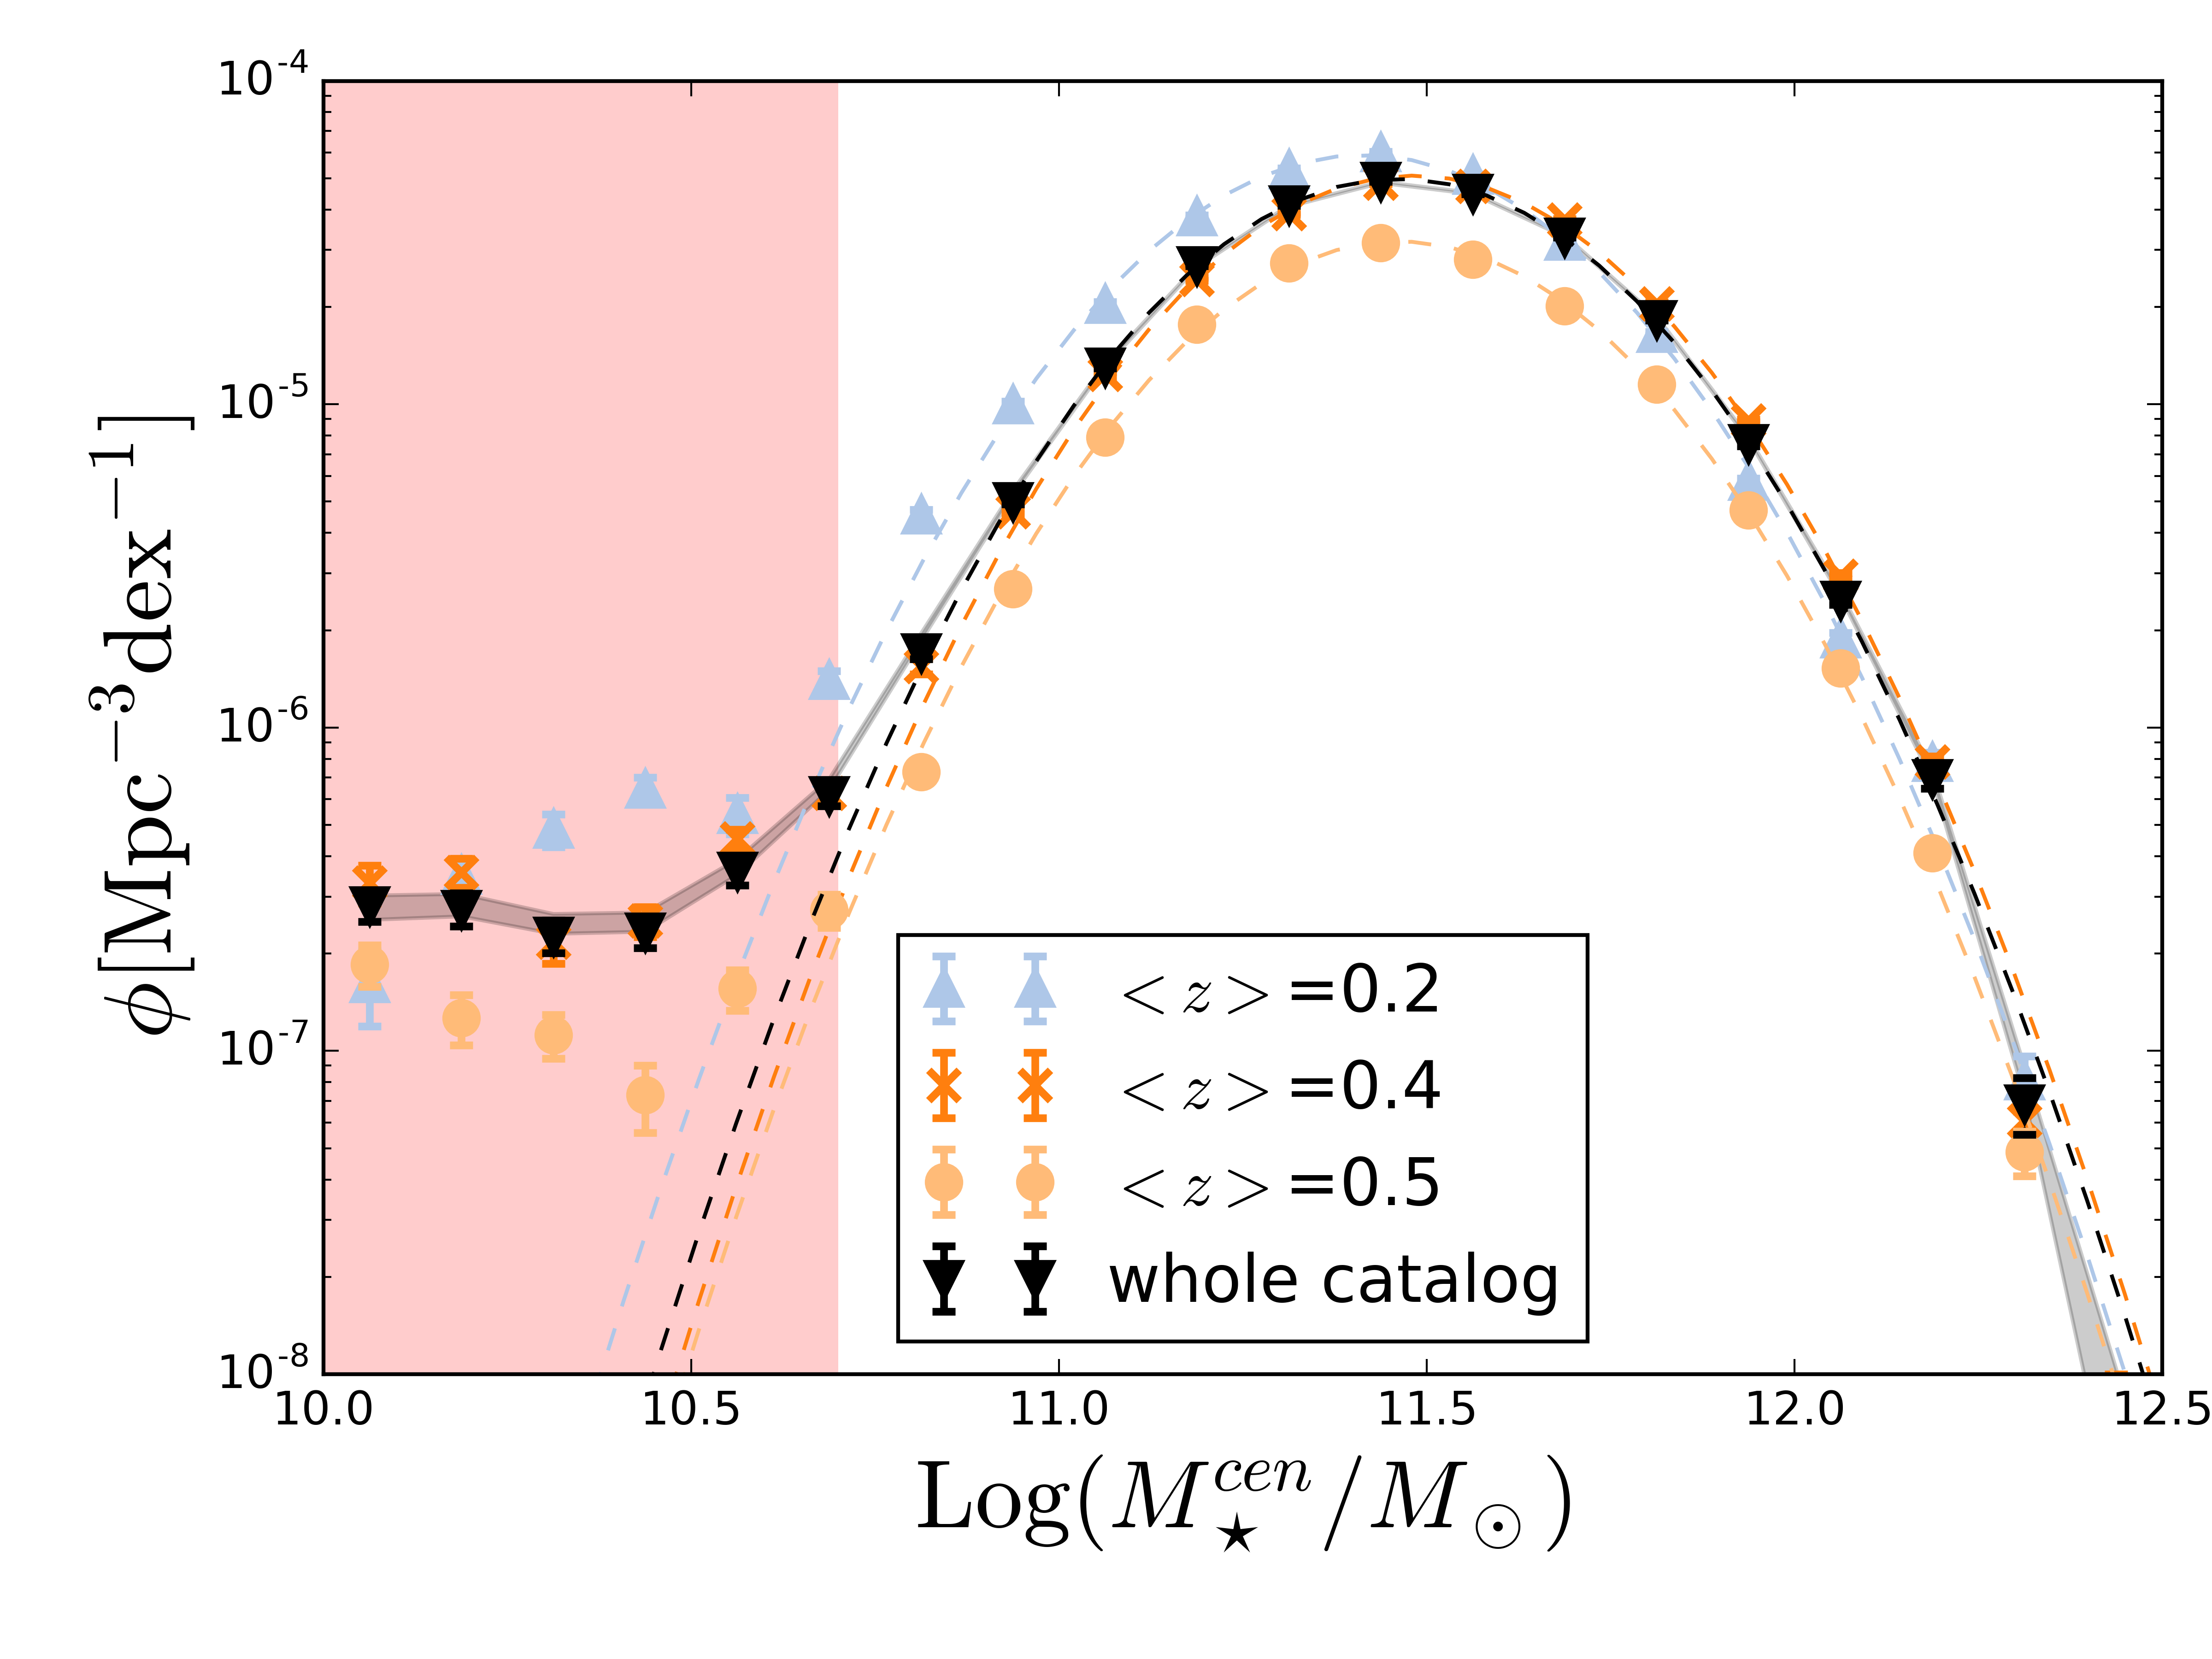
\includegraphics[width=0.7\textwidth]{./chapters/chapter6/figs/SMF_cen_chab_gaussian_Mar18.png}
\caption{Stellar mass function of central galaxies in redshift bins. Errorbars come from 200 bootstrap samples of stellar mass values for each galaxy. The dashed lines represent the best fits of these data and errors with a log--normal function. The grey region represents the 16th and 84th percentiles of the SMF from the resampling of the stellar masses to include SSP and photometric uncertainties. The red shaded region shows the part excluded in the fit.}\label{fig:smf}\end{figure}
\begin{figure}\centering
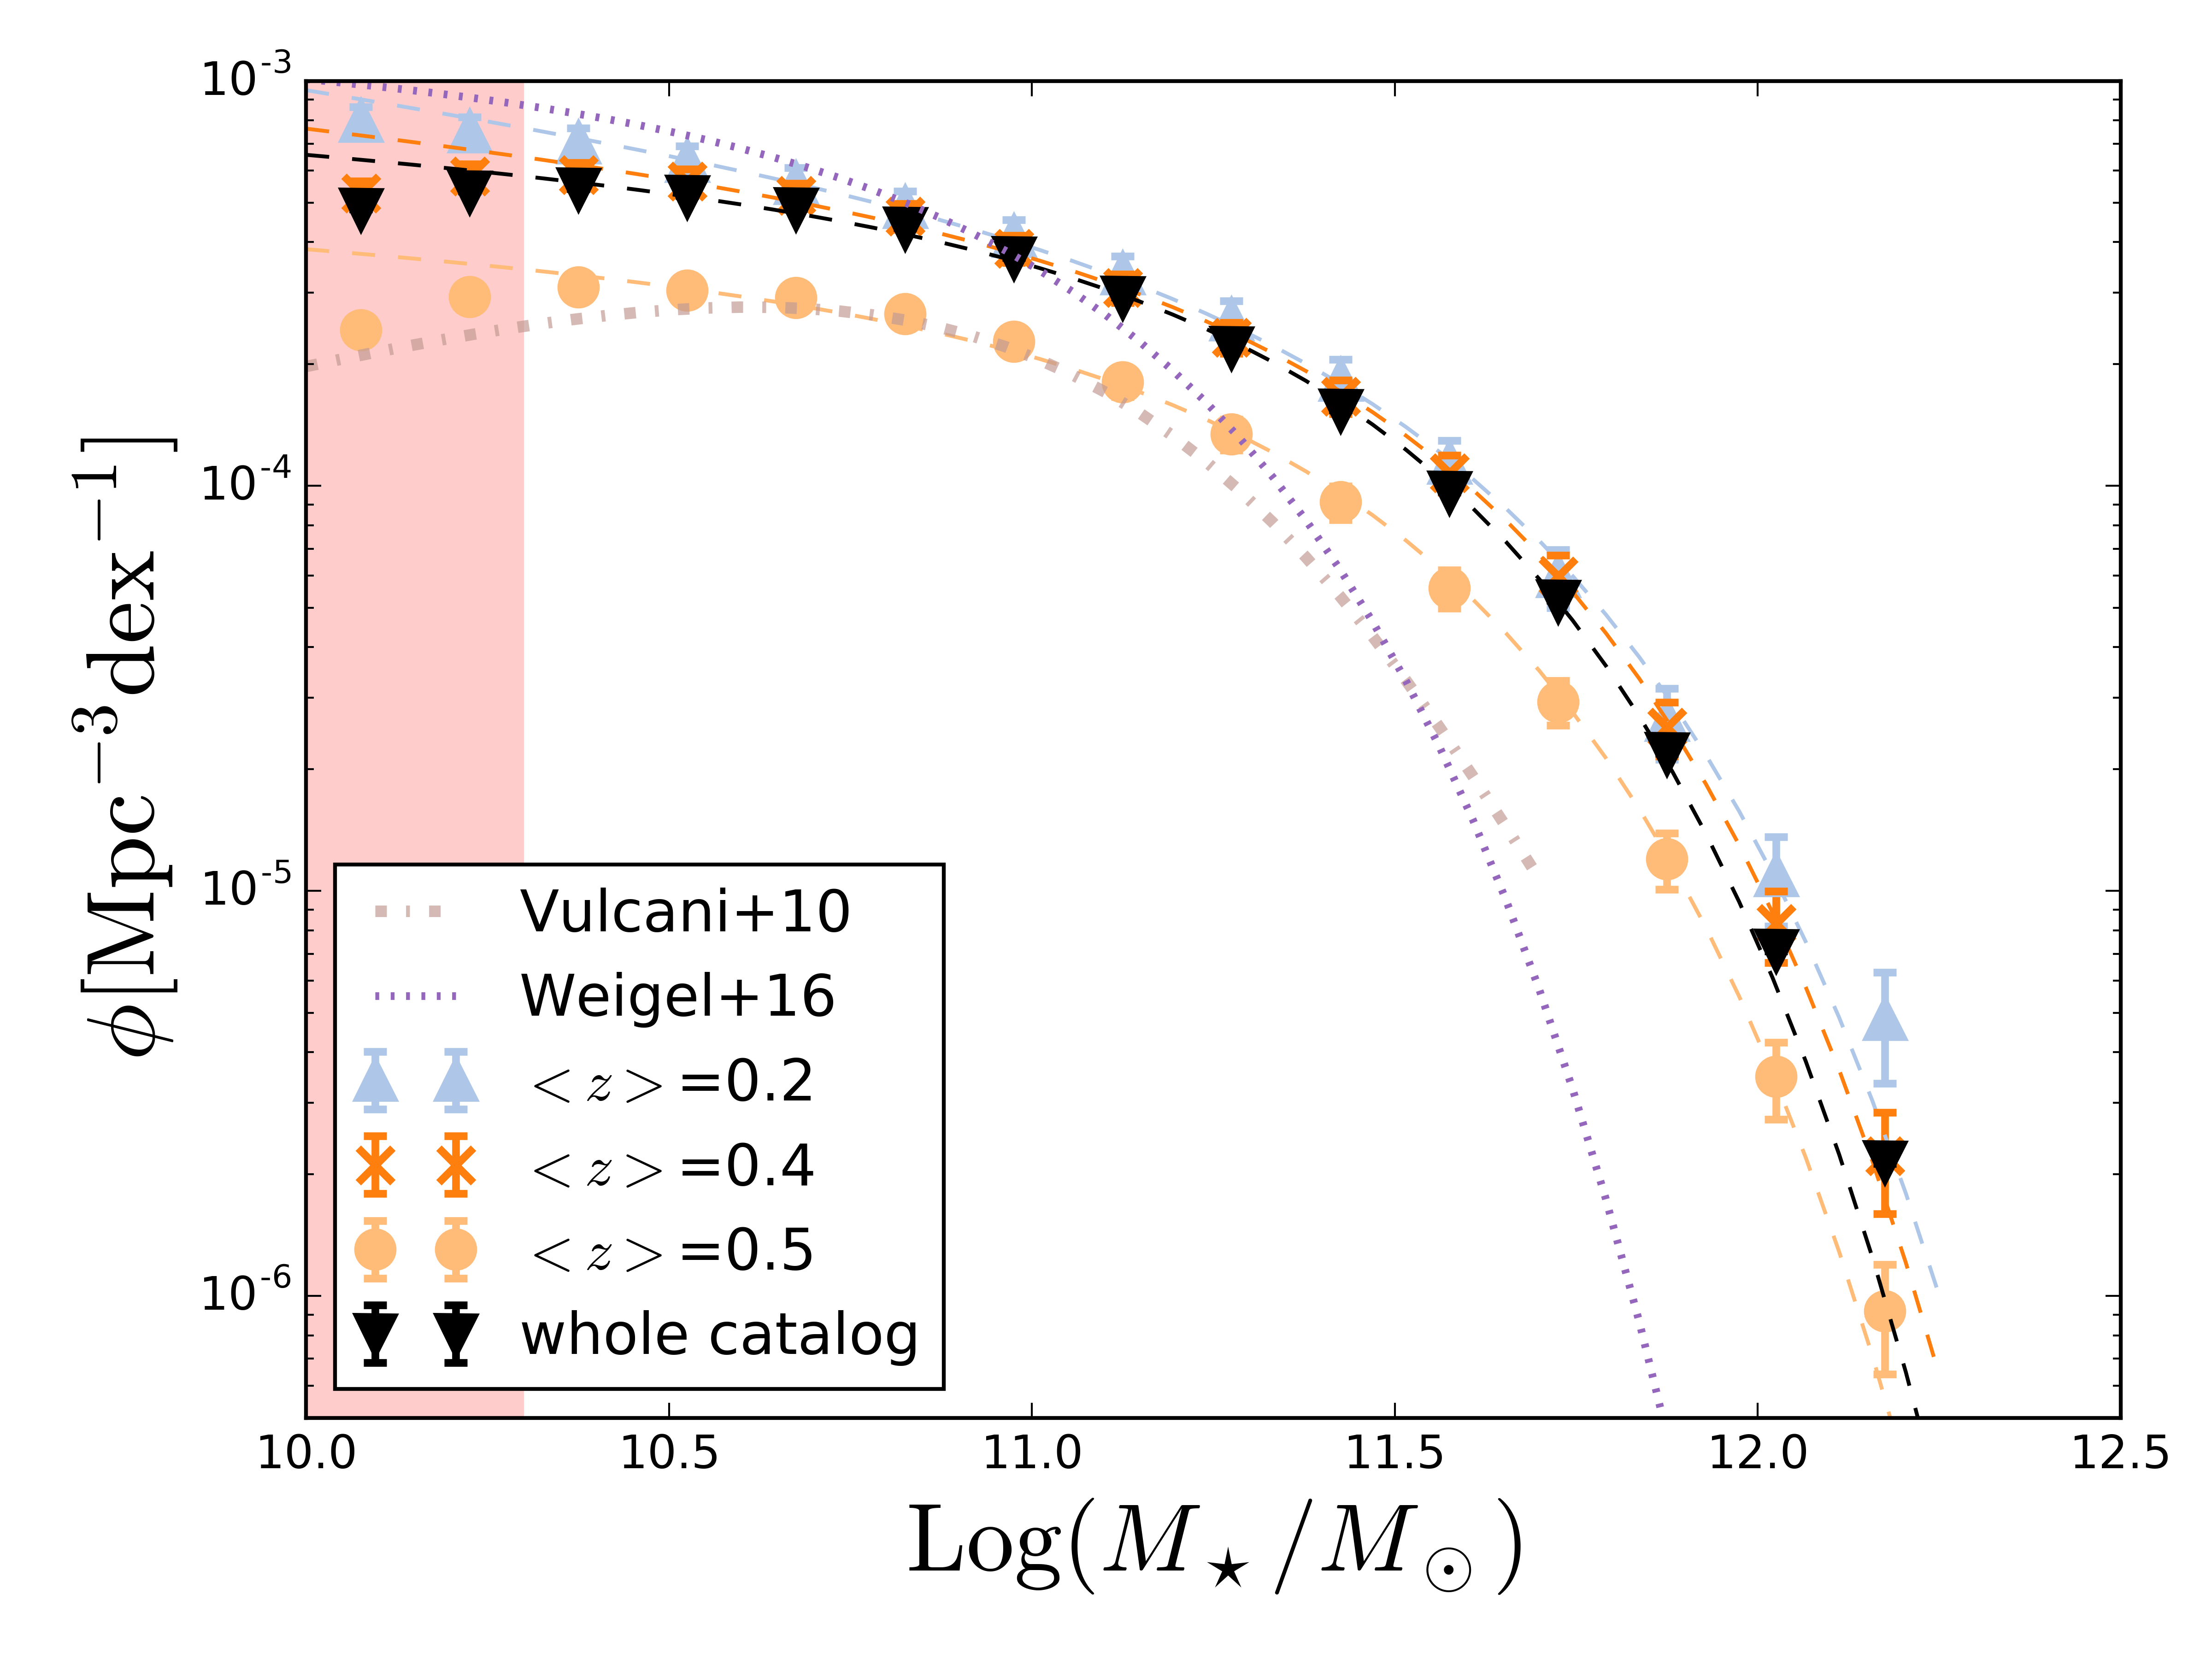
\includegraphics[width=0.7\textwidth]{./chapters/chapter6/figs/SMF_tot_chab.png}
\caption{Stellar mass function of all cluster galaxies in redshift bins. Errorbars represent the Poisson noise and the systematic error from a resampling of the stellar masses added in quadrature. The dashed lines represent the best fits of these data and errors with a single Schechter function. The red shaded region shows the part excluded in the fit. The best fit from \citet{vulcani} shown are from a sample of ESO Distant Cluster Survey clusters at $0.4<z<0.8$ for all galaxy morphological types. The dotted line is the best fit from \citet{weigel} for SDSS clusters with halo masses $13.5<{\rm Log} M_h<15$. Both distributions have been arbitrarily renormalized to match our results at ${\rm Log} M_\star =11$ at the relevant redshifts for a visual comparison of the shape of the functions.}\label{fig:smf_tot}\end{figure}

\begin{figure}\centering
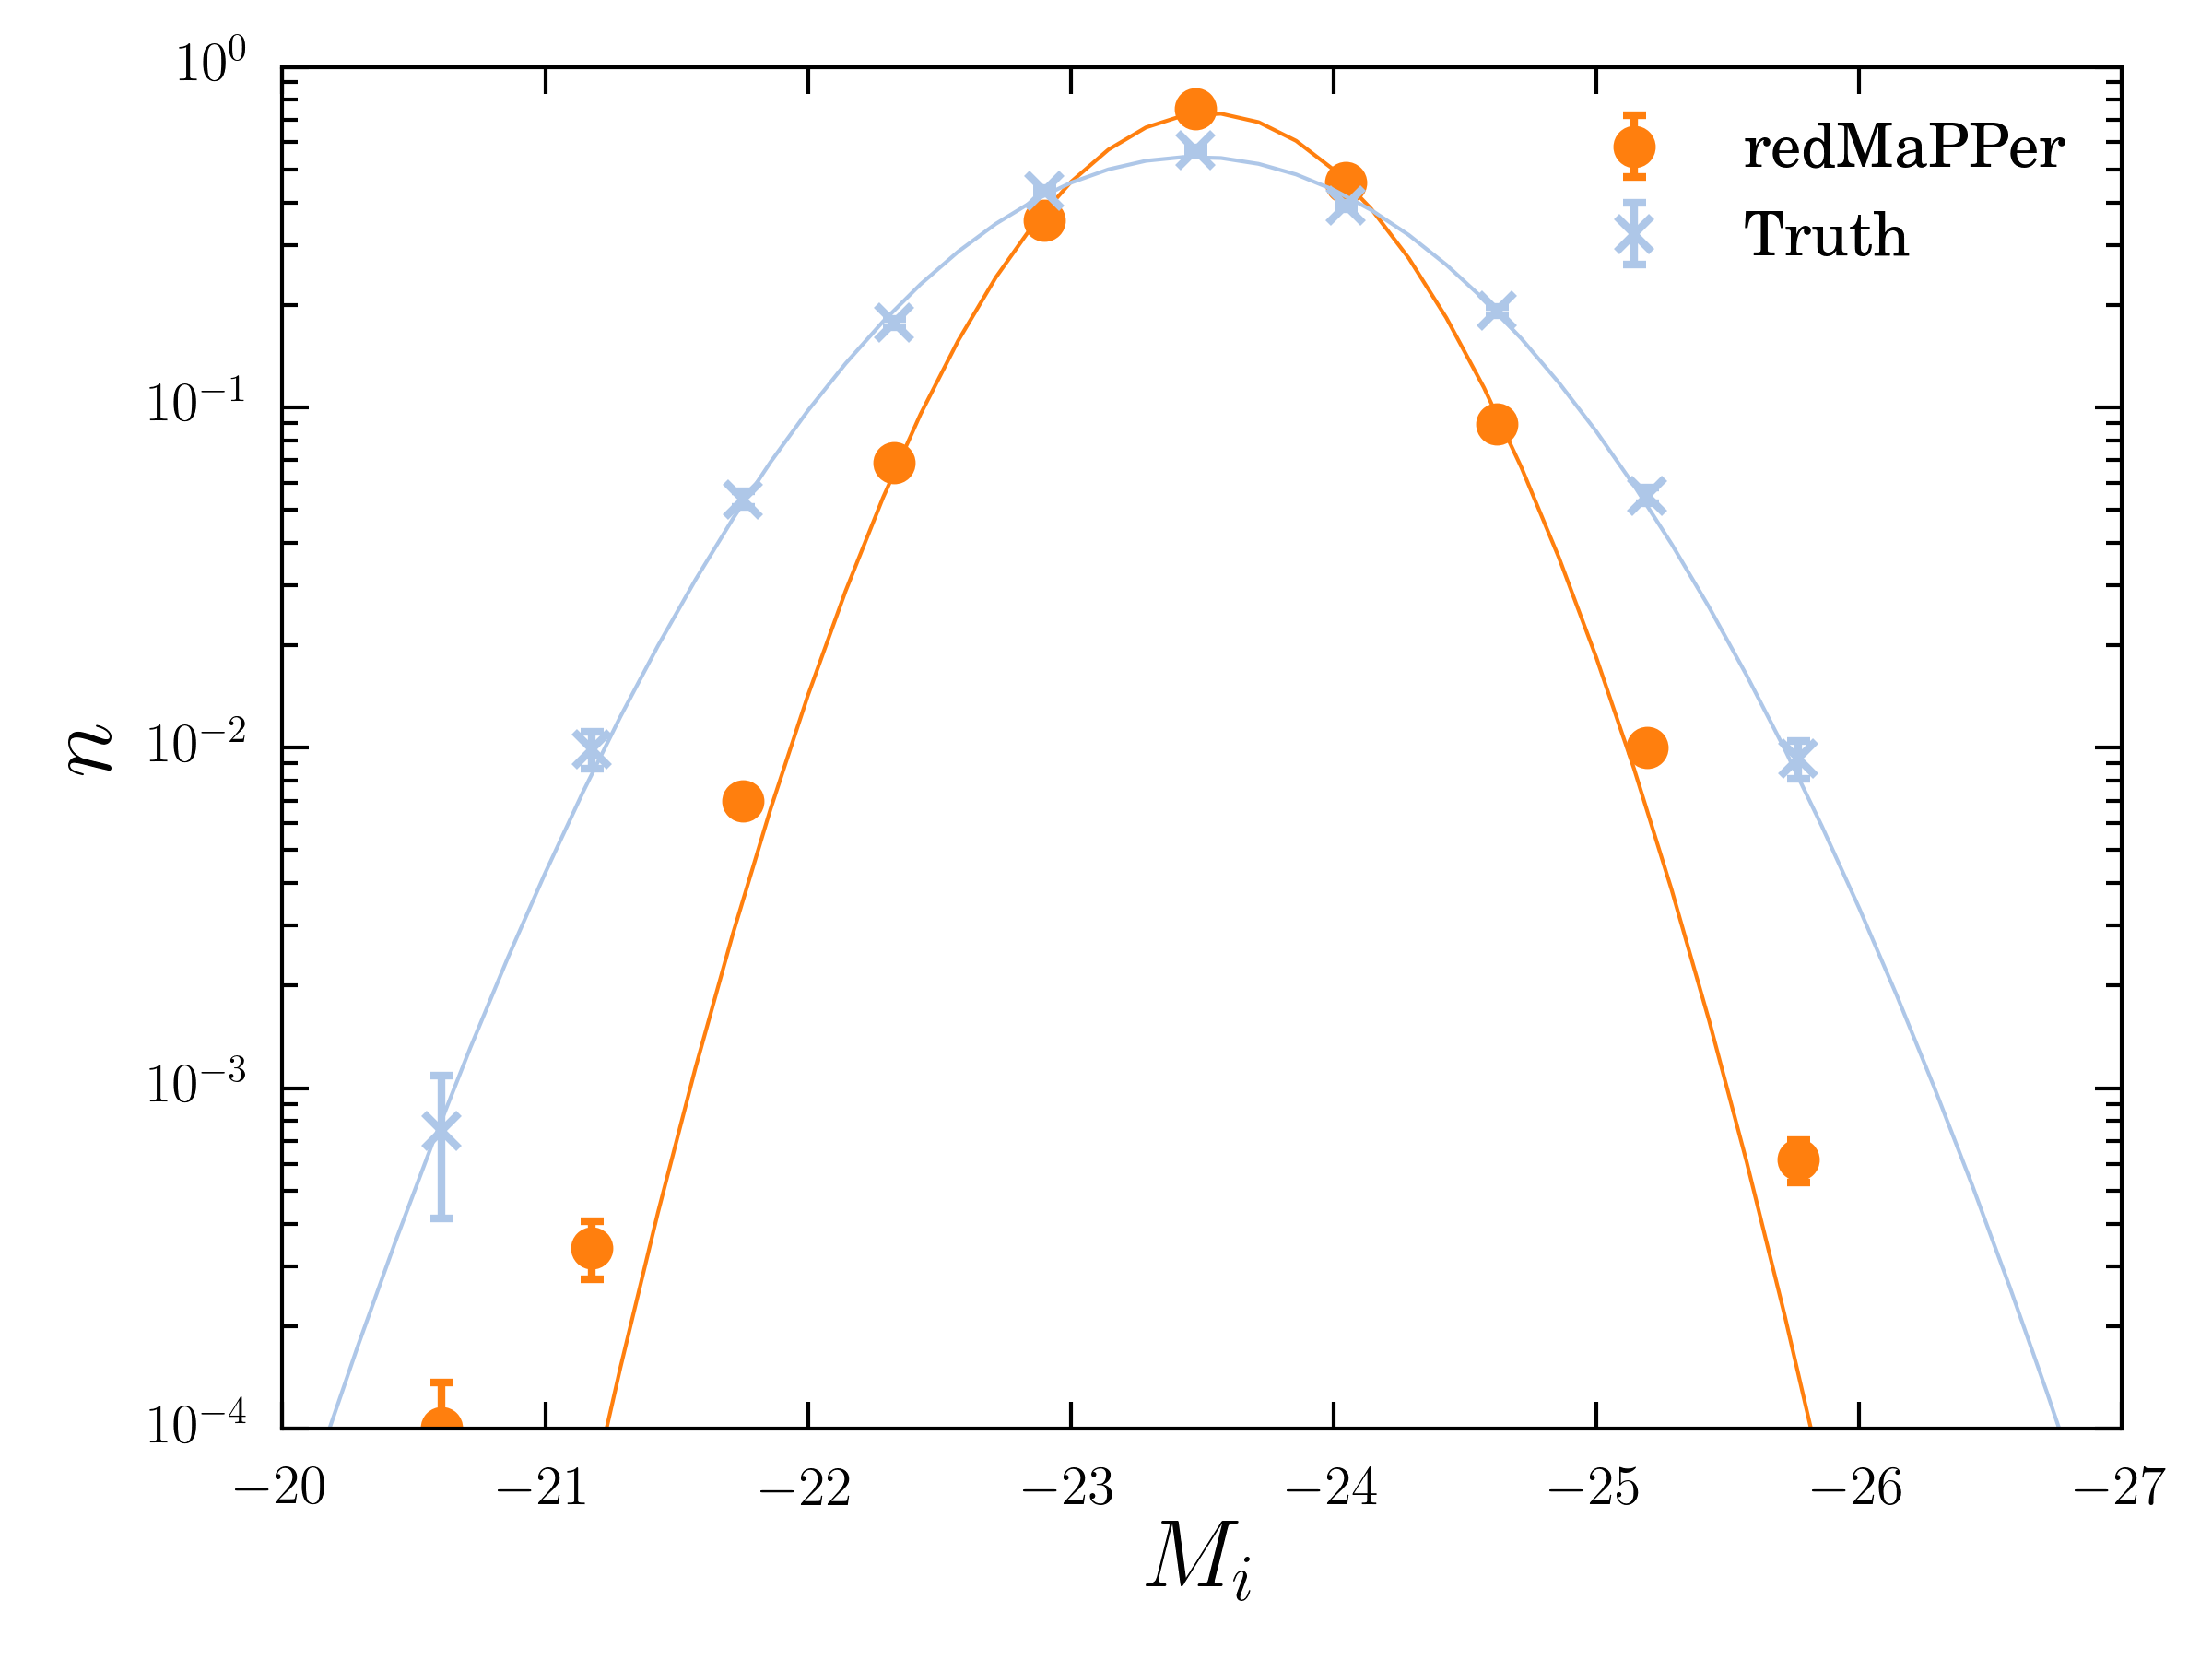
\includegraphics[width=0.7\textwidth]{./chapters/chapter6/figs/Buzzard_truth_and_red_nocuts.png}
\caption{Luminosity function of central galaxies from Buzzard simulations. The light blue data points come from the catalog of true centrals, while the orange data points represent the centrals from the redMaPPer algorithm run on the simulated data. The deviation from Gaussianity for the redMaPPer distribution is seen at the faint end. The normalisation is arbitrary. }\label{fig:smfbuzzard}\end{figure}

\subsection{Total stellar mass function}

The stellar mass function for all galaxies in the clusters is computed from the stellar mass distribution of the galaxies in our members catalog, with their entries being weighed by their membership probability. The comoving volume is computed as in the previous section for different redshift bins, and we divide the distribution by the stellar mass bin width. A Schechter function of the form: 
\begin{equation}
\phi(M) =  \phi^* e^{-M/M^*}\Big(\frac{M}{M^*} \Big)^\alpha\,,\label{eq:smf_tot}
\end{equation}
is fit to the data, with $M$ being the stellar masses for clarity of notation, $\alpha$ the parameter that controls the low-mass end slope of the SMF, $\phi^*$ a normalisation factor and $M^*$ the characteristic stellar mass at which the slope of the SMF changes significantly. Errors on $\phi$ come from adding in quadrature the statistical error from Poisson noise and a systematic error from a resampling of the galaxy stellar mass as for the centrals. Best--fit values are listed in Table \ref{tab:smf}. We exclude from the fit the bins below ${\rm Log} M_\star<10.3$ to be further from the completeness limit.
%The redshift bin containing clusters around $z\sim 0.4$ has a higher normalization value as also found in the SHMR for the same reason (see Section \ref{SHMRtot}).
It is not straightforward to compare stellar mass function measurements from different galaxy and cluster samples that used different methods and observations. In particular, the amplitude of SMF will strongly depend on the selection function of the galaxy survey considered. In this work we therefore focus on a comparing the shape of the SMF with previous literature results, where the normalization is completely arbitrary.

In Figure \ref{fig:smf_tot} we show our data points and best fit in different redshift bins and for the whole redshift range, along with the results from \citet{vulcani} for all galaxy morphological types in clusters from the ESO Distant Cluster Survey clusters at $0.4<z<0.8$. We normalize their results so that they match ours at ${\rm Log} M_\star =11$ in the lowest redshift bin. They find that the SMF is roughly flat at those redshifts, with a low--mass slope just above -1 ($-0.915\pm 0.026$), and less steep than the low--redshift sample (where $\alpha=-0.987\pm0.009$ at $0.04<z<0.07$). We also find that the slope is less steep in the highest redshift bin at $0.5<z<0.7$ ($z_{mean}\sim 0.6$), but still below -1 ($-1.108 \pm 0.034$). However, if we were to push out fit limit to lower masses, our $\alpha$ would also raise above -1. This is in fact seen when we assume a Salpeter IMF and fit over the same mass range, as this has the effect of shifting the whole distribution towards higher masses. We conclude that the discrepancy is due to different ways of dealing with the sample incompleteness. At the high mass end \citet{vulcani} have low--number statistics due to the few clusters analysed, so the SMF is not well constrained there.
%Values of $\alpha$ above unit are commonly found in cluster SMF (e.g. \citealt{yang}; \citealt{weigel})

We also plot the best fit from \citet{weigel}, who used the SDSS clusters catalogue from \citet{yang07} in the halo mass range $13.5<{\rm Log} M_h<15$. This sample partially overlaps with our lowest redshift bin ($0.1<z<0.3$), given that their cluster catalog goes out to redshift 0.2.  We normalize their results so that they match ours at ${\rm Log} M_\star =11$ in the highest redshift bin. Their low mass end slope is also below -1 ($-1.07\pm0.02$), but slightly less steep than our lowest redshift bin. In \citet{yang} they take carefully into account the cluster completeness for the same sample of \citet{weigel}, which may impact on the normalization but also the shape of the SMF (e.g. if we consider a higher fraction of high mass clusters than another analysis, we may measure a higher $M_\star$). They find that the satellites low-mass--end slope is steeper ($\alpha\sim -1.2$ to $-1.6$) than what found in \citet{weigel} at our halo masses, and satellites are the dominant contribution at the low--mass end. Our best--fit $M^*$ is $\sim 0.5$ dex above the result from \citet{weigel}, causing the discrepancy seen at the high mass end. We cannot compare to the results from \citet{yang} this value as they separate satellites from central galaxies in the conditional luminosity function, however we believe that the discrepancy is due to the cluster selection function: a qualitative analysis of the two samples shows that our volume--limited redMaPPer catalog has a fraction of clusters out to ${\rm Log} M_{200c}\lesssim 14$ which is $5-10\%$ less than what is found in \citet{yang07} catalog. This might cause the difference in the characteristic mass of the SMF.

The main conclusion of our SMF analysis is that we find evidence for an evolution of the low--mass end slope over the redshift range $0.1<z<0.7$, and no or little evolution at the high--mass end. This implies that the population of low mass galaxies evolved significantly since redshift 0.7, while the mass build-up of the more massive galaxies has mostly been completed by then.  Given the absence of evidence for redshift evolution seen in the previous subsection, the behaviour observed at the massive end includes the centrals.

%, while for the overall distribution the 


\begin{figure}\centering
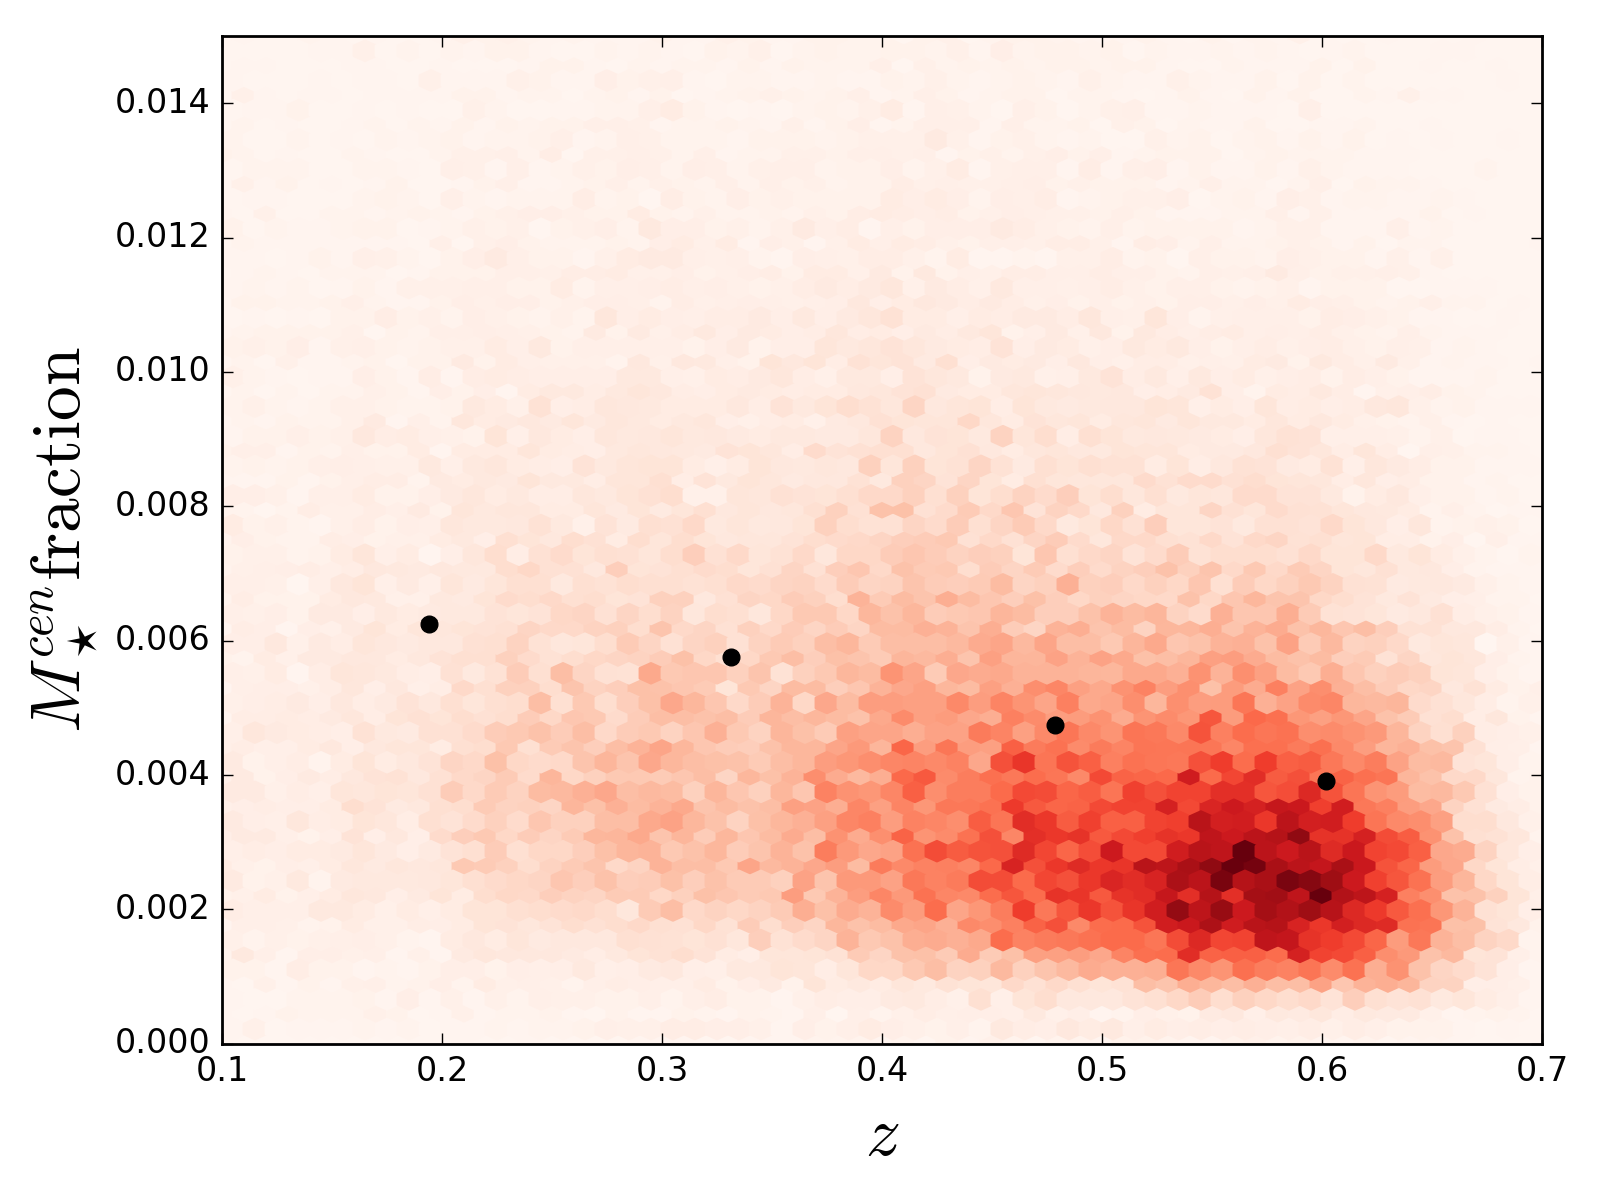
\includegraphics[width=0.7\textwidth]{./chapters/chapter6/figs/BCG_growth.png}
\caption{Central mass growth with redshift. The stellar masses are divided by the corresponding cluster halo mass at $z=0$ for a comparison of different clusters. The data points represent the mean stellar mass fractions in redshift bins. }\label{fig:mcengrowth}\end{figure}

\begin{figure}\centering
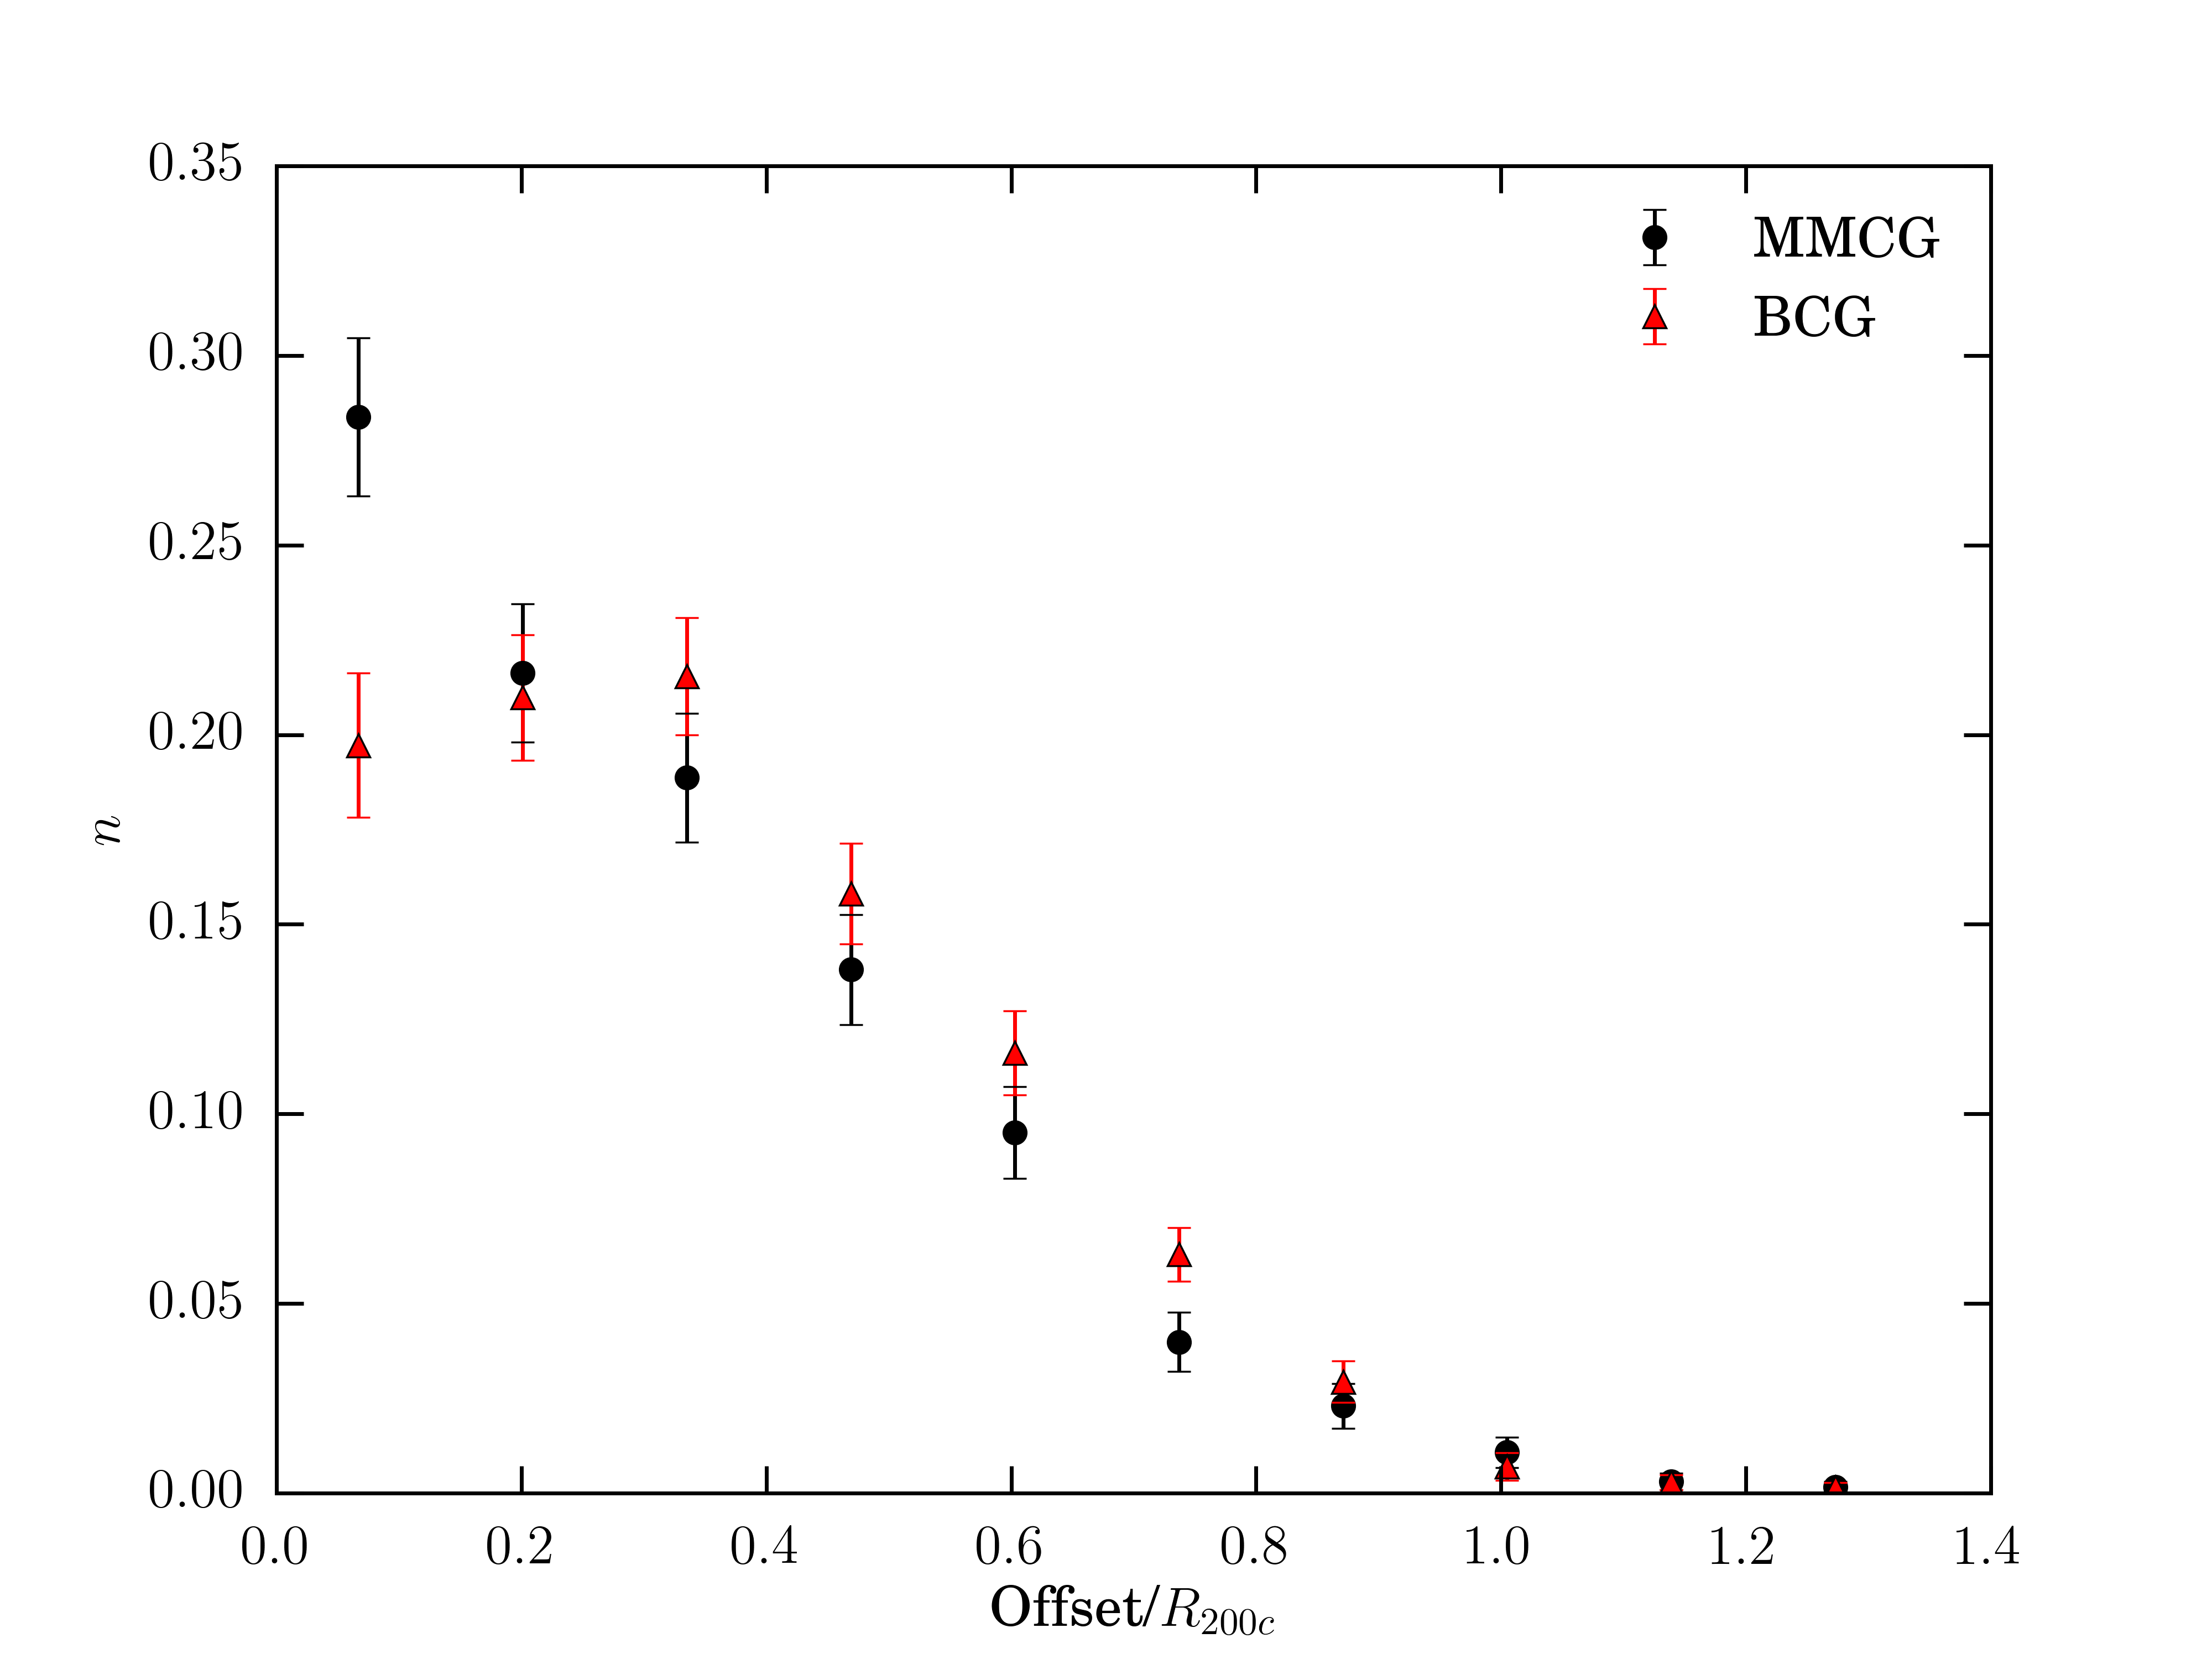
\includegraphics[width=0.7\textwidth]{./chapters/chapter6/figs/offsets.png}
\caption{Distribution of the offsets from the redMaPPer central for the most massive cluster galaxy (black points) and the brightest cluster galaxy (red triangles) when they do not coincide. Errorbars are given by the Poisson error.}\label{offsetsfig}\end{figure}

\section{Mass growth and definition of centrals}\label{sec:centrals}

\subsection{Central stellar mass growth}\label{sec:cengrowth}

While semi-analytic models (\citealt{delucia}) predict BCG stellar mass growth of the order of 4 between redshift 1 and 0, observations seem to be in contrast. \citet{lidman} found an increase of $\sim 1.8$ between $z=0.9$ and $z=0.2$. We follow a similar method and correct the stellar mass of the central in order to take into account for the correlation with the mass of the halo it belongs to. %This is crucial because of our sample selection: we observe higher halo masses at higher redshift in this case, and we therefore want to correct for it. 
When we correct the BCG mass using the $M_{200c}$ estimate from the weak lensing calibration we find no evidence of stellar mass growth between redshift 0.7 and 0.1. It follows that the mild redshift evolution found in Section \ref{shmrsec} for the SHMR of centrals is due to a different cluster selection function at different redshifts. Correcting by the halo mass that the cluster would have today brings to a different result. We use the mean accretion rate from \citet{accretion} to extrapolate the mass of the clusters from the redshift at which they were observed to the current time. The results are shown in Figure \ref{fig:mcengrowth}. Between redshift 0.7 and 0.1 we find a growth of a factor $\sim 1.6$: as expected due to the significant mass accretion of halos from redshift 1, the central mass growth is higher when correcting for the halo mass as it would be today. On the other hand, the scatter in the mass fraction is considerably high, $\sim 30-50\%$ in each redshift bin. This result corresponds to a $\sim 0.2$ dex growth, which is consistent with $0.29\pm0.11$ dex between $z=1$ and $z=0$ found by \citet{zhangbcg} for the cluster sample with ${\rm Log}(M_{200c}) >13.85$ (the lowest mass systems are excluded due to uncertainties in the X-ray temperature--mass relation).

\subsection{Definition of central, BCG and most massive galaxy}
%Codes in des60.b lambda_star/redmapper_y1a1/lambda5

So far we have considered redMaPPer centrals in comparison with results from some studies of BCGs, as if they were the same objects. Identifying and in case discerning between these two components is not always trivial because galaxies in the core of the cluster are moving at speeds of $\sim 200$ km/s and also will undergo  merging and stripping events. 

We  identify the BCG as the brightest galaxy in $i$-band absolute magnitude and the most massive cluster galaxy (MMCG) as the galaxy with the highest stellar mass. The latter should also roughly correspond to the  BCG if we consider that most of the giant red galaxies close to the cluster core  have similar mass-to-light ratios. In order to select the possible candidates, we use $N  = \Sigma_i p_{\rm mem}$ to estimate the number of galaxies $N$ in each cluster, where the sum goes over all the galaxies associated with the cluster.  Only galaxies in the highest 40th percentile of the $p_{\rm mem}$ distribution  are considered, in order to avoid considering galaxies that are not associated with the cluster.
We find that $\sim 24\%$ of clusters have a MMCG that is not the redMaPPer central, and $\sim 30\%$ have a BCG which is not the central. If the redMaPPer centre is given as a truth table, then the most massive galaxy traces better the central than the brightest. We can interpret this result in terms of abundance matching. If there were no scatter in the halo-galaxy abundance matching, then this statement would always be true: the galaxy with most stellar mass would also be the central as its sub-halo would be the most massive among all sub-halos. In reality, the existing scatter between stellar mass and sub-halo mass impacts on the one-to one relation between those two quantities and the MMCG will not always be the central. Similarly, \citet{hoshino} found that $20-30\%$ of SDSS redMaPPer centrals are not the brightest Luminous Red Galaxies (LRGs) in the cluster. The offset distribution of the MMCGs and BCGs compared to the redMaPPer centers are shown in Figure \ref{offsetsfig} for those clusters in which MMCG (or BCGs) and centers do not correspond. 


\begin{figure}\centering
\includegraphics[width=0.63\textwidth]{./chapters/chapter6/figs/Imfs.png}\caption{Most commonly used Initial Mass Functions. Note that the Salpeter IMF diverges at the low-mass end. }\label{fig:imf}
\end{figure}

\section{Impact of the Initial Mass Function}\label{sec:imf}
The choice of the IMF is regarded as one of the main cause of systematics in stellar mass estimation (\citealt{coupon}). The IMF describes the distribution in mass of the stars when they enter the main sequence. It is given as the number of stars that have been born with initial stellar masses between $M_\star$ and $M_\star+{\rm d} M_\star$: $\xi(M_\star) {\rm d} M_\star$. Some of the most used IMFs are shown in Figure \ref{fig:imf} and are defined as:
\begin{itemize}
\item \citet{salpeter}: $\xi(M_\star)=k M_\star^{-2.35}$, where $k$ is a normalization factor.
\item \citet{kroupa}: $\xi(M_\star) = k M_\star^{-\alpha}$, where \begin{equation}
\alpha = \left\{ \begin{array}{ll}   0.3 & {\rm if} ~M_\star < 0.08\\
1.3 & {\rm if} ~0.08<M_\star < 0.5\\
2.3 & {\rm if} ~M_\star >0.5\\
\end{array}
\right.
\end{equation}
\item \citet{chabrier}:
\begin{equation}
\xi(M_\star)= \left\{ \begin{array}{ll}   \frac{0.158}{{\rm ln}(10)M_\star} {\rm e}^{-\frac{({\rm Log}(M_\star) - {\rm Log}(0.08))^2}{2\times 0.69^2}} & M_\star < 1\\
kM_\star^{-2.3} & M_\star > 1
\end{array}
\right.
\end{equation}
where $k$ is a normalization factor.
\end{itemize}
The \citet{kroupa} and \citet{chabrier} IMFs are representative of the IMF in the Solar neighbourhood, and the \citet{salpeter} one is considered a dwarf--rich or bottom--heavy IMF, as it deviates from the others at $M_\star<1 M_\odot$.

Most works report their results assuming a Chabrier IMF, but several studies (e.g. \citealt{imf13}, \citealt{imf151}, \citealt{imf15}) have shown that the IMF of massive elliptical galaxies is better described by a more bottom-heavy function. If that is the case, SHMR may be biased (\citealt{kravtsov}) at all halo masses, as a result of the stellar mass estimates being biased for most of the red sequence galaxies. So far we have assumed a Chabrier IMF for a more straightforward comparison with other literature results. Here we reproduce the same analyses assuming a Salpeter IMF in the SSP models used to fit the stellar mass. This represents the extreme case of an IMF diverging at the low mass end: the difference between the SHMR obtained by assuming a Chabrier and a Salpeter IMF will give us an estimate of the systematic uncertainty due to the uncertainty on the IMF. In Table \ref{fitstable} we report the results for the SHMR when assuming a Salpeter IMF, and in Table \ref{tab:smf} for the SMFs. This different IMF has the effect of biasing the galaxy and the cluster stellar masses, resulting in a change in the intercept of the linear relation between halo mass and stellar mass, and in the mean of the centrals SMF log--normal fit. Table \ref{fitstable} shows that the pivot ${\rm Log}(\tilde{M}_\star)$ is 0.23--0.27 dex higher in the case of a Salpeter IMF.
\citet{kravtsov} find that the effect of a more bottom-heavy IMF steepens the SHMR, as they study this effect by introducing a mass-to-light ratio which depends on the velocity dispersion in galaxies (and therefore on their total mass). In our work we are assuming the same IMF for all galaxies, as our SED fitting of photometric optical data would not be able to distinguish between different IMFs, and most of the cluster stellar mass is contributed by the old elliptical galaxies. This measurement gives us the most conservative upper limit to the SHMR and SMF. Our results is remarkably consistent with \citet{2012ApJ...746...95L}, who find a 0.25 dex shift in the $f_\star-M_{\rm halo}$ relation due to changing IMF from a Chabrier to a Salpeter.


%%% Add comparison when we have f* fraction too: kravstov finds increase in the tot f* by a factor 1.6-1.7 or by 0.04-0.06 in absolute values in units of omb/omm. for centrals it increases by a factor 1.5-2. This may explain some of the missing baryons they say??? They also claim that the high mass haloes are not so much less efficient in converting baryons into stars compared to L* gals.


\section{Intra-cluster light}\label{sec:icl}

\subsection{Colour and stellar mass}
\begin{figure}\centering
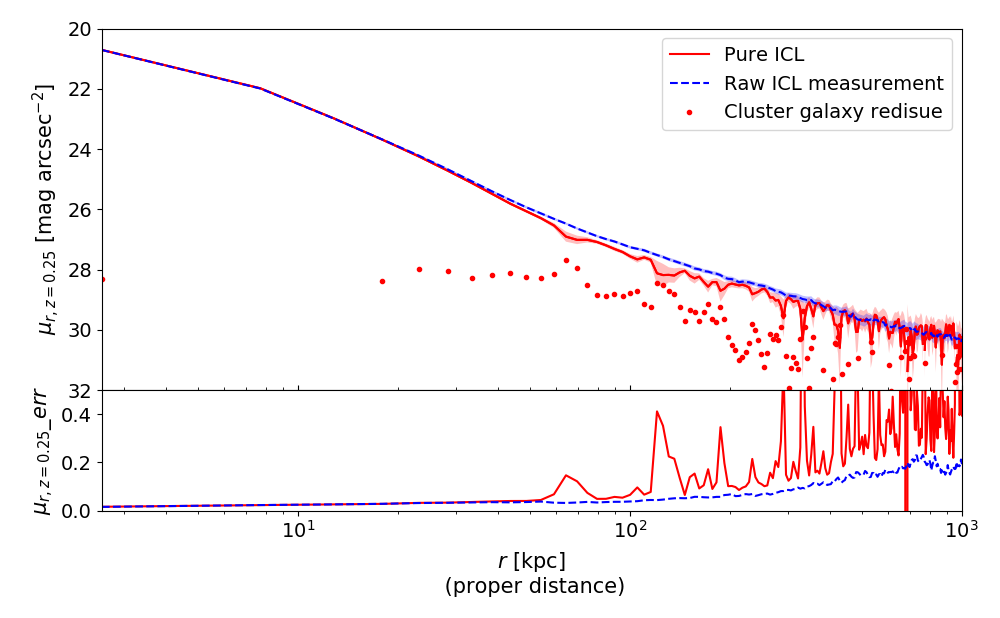
\includegraphics[width=0.7\textwidth]{./chapters/chapter6/figs/icl.png}
\caption{This figure shows the derived ICL profiles (upper panel) and the uncertainties of the measurements (lower panel). Cluster galaxy residue (red point) is subtracted from the raw ICL measurements (blue line) to derive pure ICL profile (red line). Uncertainties of the ICL profiles are displayed as the shaded regions (upper panel) and also shown in the lower panel against radii. The ICL profiles are measured with high S/N to 1 Mpc, despite the subtraction of cluster galaxy residue introduces significant noise into the profile. Plot by Yuanyuan Zhang.}
\label{fig:cluster_profile}
\end{figure}
\begin{figure}\centering
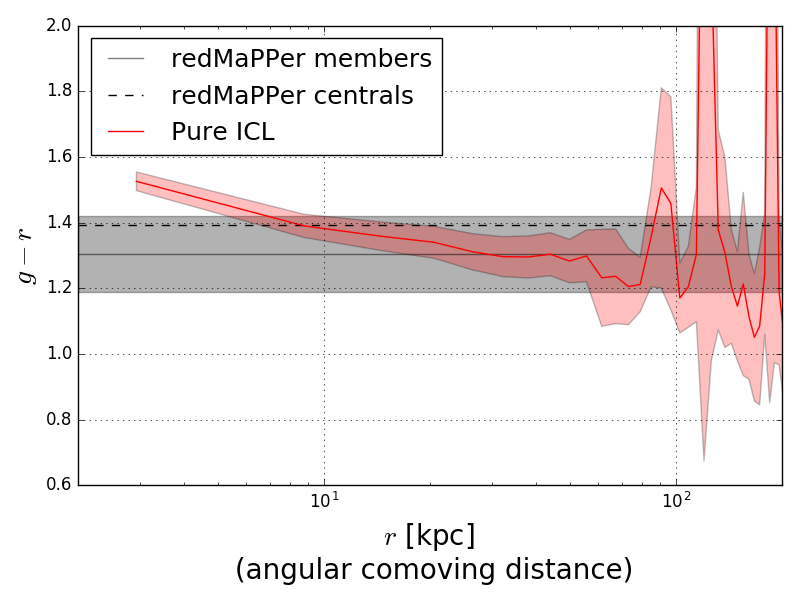
\includegraphics[width=0.7\textwidth]{./chapters/chapter6/figs/icl_color.png}
\caption{Colour Profile of pure ICL. Errors are computed with the Jackknife method. The horizontal lines are the mean redmaPPer colours (K-corrected to $z=0.25$) from the redMaPPer cluster members at $0.2<z<0.3$ and their central galaxies. The shaded region around the members' colour mean represents 1 standard deviation of the sample.}
\label{fig:color}
\end{figure}

In Section \ref{SHMRtot} we mentioned that the ICL can contribute up to $\sim 40\%$ of the total cluster stellar mass. This statement is based on ICL measurements from the DES data. Through averaging $\sim300$ galaxy clusters from the DES Y1 redMaPPer catalog, in \citet{icl} we report the detection of diffuse intra-cluster light at a surface brightness limit of 30 mag/arcsecond$^{2}$ to 1 Mpc in DES $r-$band. The analysis is further verified by averaging the images of random points and point-like sources. After estimating the light from cluster galaxies, we infer that the diffused intra-cluster light associated with the cluster central galaxies extend to 200 kpc and beyond. This diffuse light constitutes a significant component of the central galaxy light: light contained beyond 32 kpc makes up $\sim 42\%$ of the total light within 200 kpc. In Figure \ref{fig:cluster_profile} we show the derived ICL profiles (upper panel) and the uncertainties of the measurements (lower panel). Cluster galaxy residue (red point), excluding the central galaxy, is subtracted from the raw ICL measurements (blue line) to derive a ``pure'' ICL profile (red line). The pure ICL profile therefore contains the contribution of the central galaxy and the diffuse stellar matter, given that there is no clear separation between the two components.  Uncertainties of the ICL profiles are displayed as the shaded regions (upper panel) and also shown in the lower panel against radii, where the errors are computed through a jackknife resampling of 40 regions. The ICL profiles are measured with high S/N to 1 Mpc, despite the subtraction of cluster galaxy residue introduces significant noise into the profile.

We further derive the ICL colour profile of $g-r$, utilizing our measurements of ICL profiles in the $g-$band. The result is shown in Fig. \ref{fig:color}. We find that the mean colour of pure ICL becomes bluer at larger radii. A $\chi^2$ minimization gives a gradient $\nabla (g-r) \equiv \frac{{\rm d} (g-r)}{{\rm d \, Log}(r)}=-0.203\pm 0.011$ within the inner 90 kpc, showing a negative colour gradient at a $18\sigma$ level. If we only consider the range $10<r<90$ kpc, therefore excluding the central part of the CG we find $\nabla (g-r) =-0.152\pm 0.027$. The result is consistent with previous works (e.g. \citealt{demaio}) on ICL colour gradient in individual clusters, although there exist clusters that does not display this trend. Note that the ``spikes'' in Figure \ref{fig:color} are a consequence of our measurements. In fact, these are present in the pure ICL profile from Figure \ref{fig:cluster_profile}, and come from the galaxies profile which is subtracted from the ``raw'' ICL measurement. The spikes show up at the galaxies' positions. The $g-$band profiles are even fainter and noisier than those in $r--$band, and thus are more visible in the colour profile.

In Figure \ref{fig:color}, we also show the colours of cluster central and satellite galaxies for comparison to ICL. Those are the mean colours from \texttt{MODEL\_MAG} magnitudes, K-corrected to $z=0.25$ as done for the ICL. While in the inner $\lesssim 10$ kpc the ICL is as red as most central galaxies, outside this range it appears to be consistent with the cluster satellite galaxies. This result, together with ICL getting bluer at larger radii, indicate that in the inner tens of kpc the central galaxy blends in the ICL profile, and in the outer regions the ICL build--up channel is likely dwarf disruption and tidal stripping. In fact, the former mechanism is expected to create a colour gradient as the disrupted dwarfs lived at different radii depending on their mass (and therefore on their colour). On the other hand, tidal stripping will be stronger closer to the cluster center and will be able to strip the redder, inner parts of the cluster galaxies. Major mergers are not likely to be the main ICL formation mechanism, as this would give rise to more uniform colour profiles (e.g. \citealt{2013A&A...553A..99E}). 

\begin{figure}
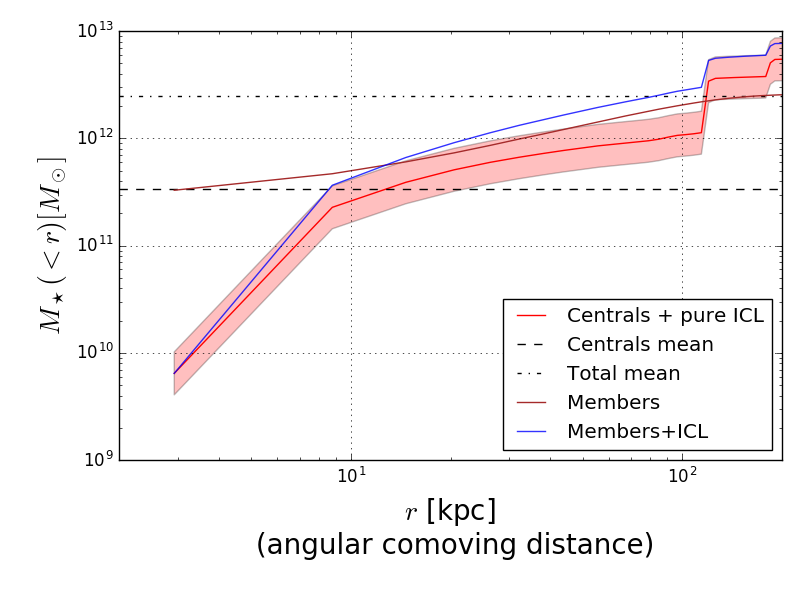
\includegraphics[width=0.5\textwidth]{./chapters/chapter6/figs/mtot.png}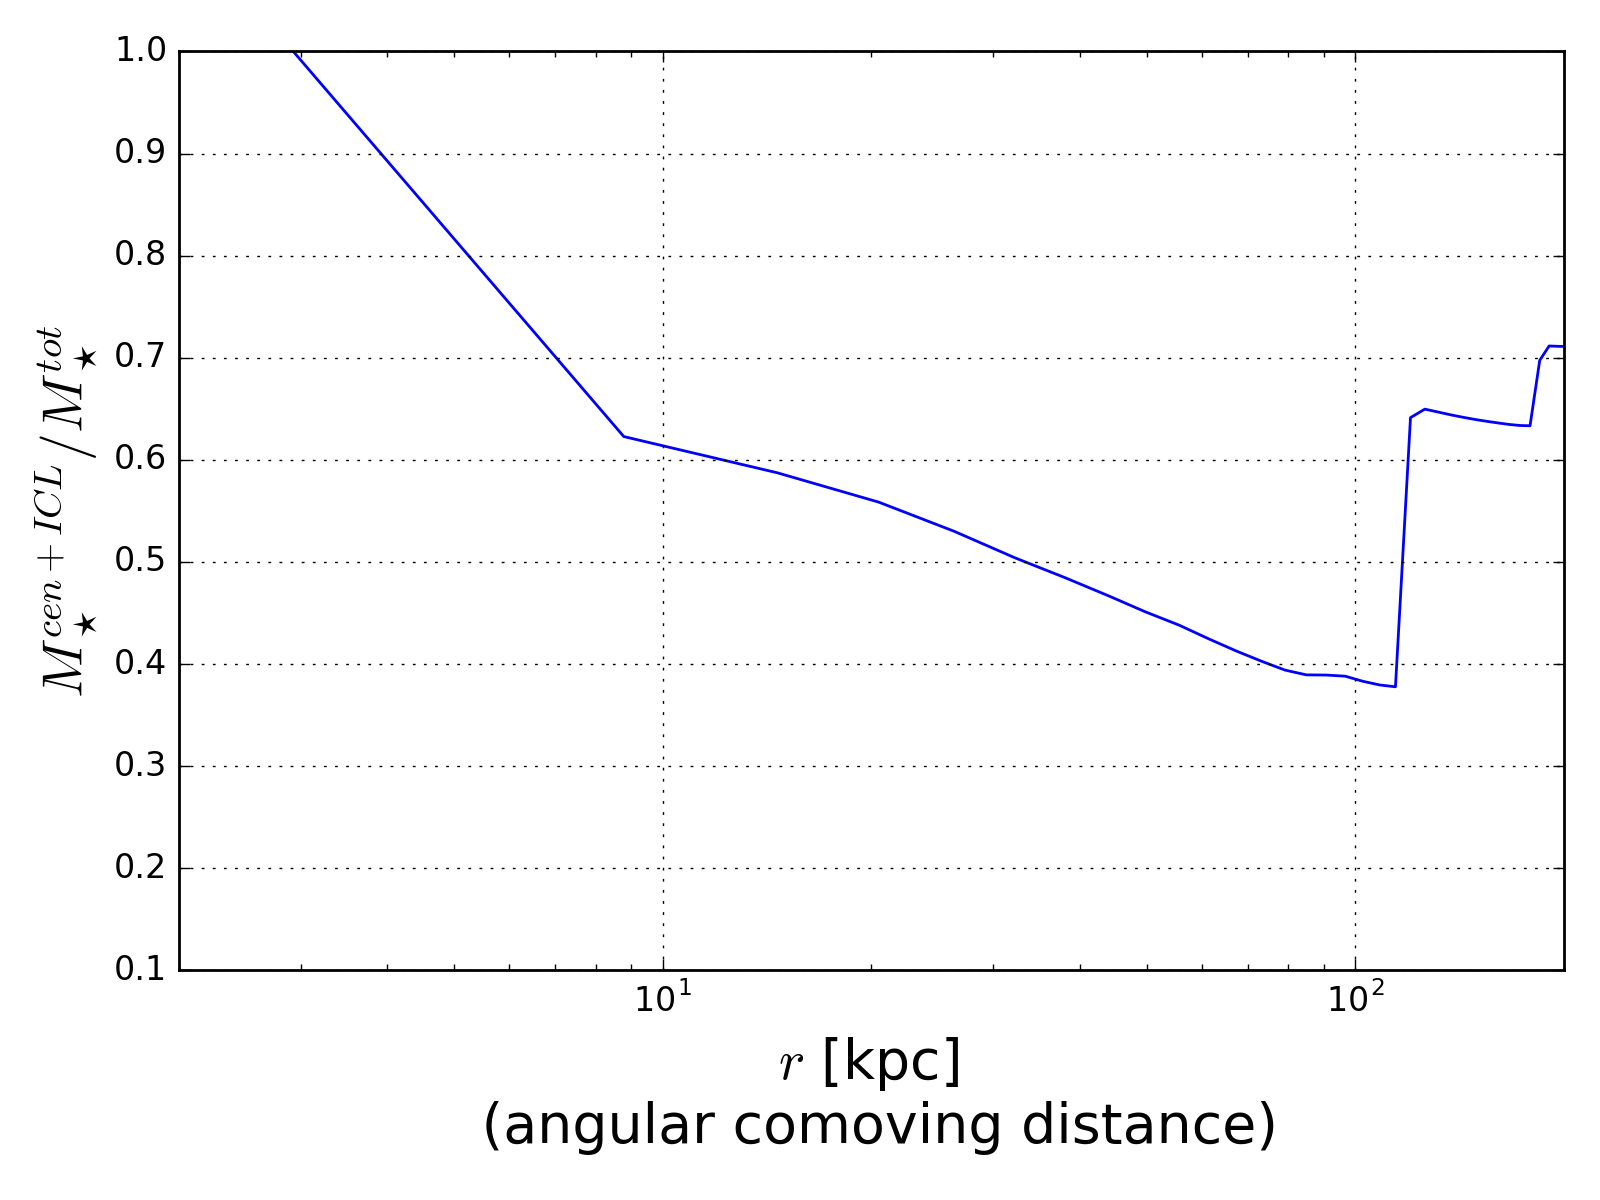
\includegraphics[width=0.5\textwidth]{./chapters/chapter6/figs/mstar_fraction.png}
\caption{Left: Cumulative stellar mass profile contribution of different cluster components for DES clusters at $0.2<z<0.3$. Right: Fraction of stellar mass that resides in the central plus the pure ICL as a function of radius. These measurements are too sensitive to the noise in the galaxies profile subtracted from the raw ICL profile beyond 100 kpc, we thus can only base our analysis below that value. }
\label{fig:icl_mstar}
\end{figure}

From the $g$ and $r$ profiles we can also derive stellar mass profiles. We use the relation between colour and mass-to-light ratio in $r-$band derived in \citet{bell}: ${\rm Log} (M_\star/L_r) = 1.097 (g - r) - 0.306$.  This equation has been derived for $g$ and $r$ SDSS filters, but the difference in the magnitudes brought by the use of DES filters is negligible compared to the typical errors in the stellar mass.  These values have been corrected by 0.1 dex to provide estimates consistent with a Chabrier IMF, while \citet{bell} used a corrected Salpeter IMF. The $M/L$--colour relation is used at all considered radii to derive a stellar mass surface brightness profile $\Sigma_\star=M/L_r \times \Sigma L_r(R)$. Luminosities are estimated from the absolute magnitudes $M_r$ derived from the apparent magnitude $r$ as $M_r = r - k_{rr} -EC(z) -DM$ where $k_{rr}$, $EC(z)$ and $DM$ are the $K$-correction, the evolutionary correction and the distance modulus respectively. Similarly it is done for $g$ band. The evolutionary correction used is from \citet{bell}: $EC(g, r) \sim (-1.6, -1.3)z$, and the conversion from magnitudes to luminosities in $L_\odot$ units is performed using the absolute magnitudes of the Sun $M_{g,\odot} = 5.15$ and $M_{r,\odot} = 4.67$. Here we show results for the $r-$band as it is less noisy than the $g$ band. In Figure \ref{fig:icl_mstar} we show the cumulative stellar mass profiles obtained in this way, and compare to the stellar mass results computed as described in Chapter \ref{chp:sed} and Chapter \ref{chp:proxy} with the BMA method. From the Y1 redMaPPer sample, we only select the same clusters used for the ICL detection for this comparison. The profile of the central galaxy plus the pure ICL is shown in red, with the shaded region being the error. Jackknife errors on the measured fluxes have been propagated to the stellar mass with the error propagation chain. This measurement is too sensitive to the noise in the galaxies profile subtracted from the raw ICL profile beyond 100 kpc, and we therefore restrict the analysis to this radius. This profile is comparable to the mean stellar mass value of centrals (dashed line) in the range $8~{\rm kpc} \lesssim r \lesssim 30$ kpc, showing that our stellar mass estimates from the MOF photometry are able to recover the diffuse ICL component within this range on average. The brown line represents the profile from member galaxies in our cluster catalog with masses computed through the BMA method. Clearly in this case the mass of the central is considered at 0 kpc from the centre instead of being an extended component, explaining the discrepancy at low radii. We also show the mean value of the total (i.e. from all members) mass within 200 kpc. It is interesting to understand what fraction of the total stellar mass is in the ICL component. This is shown in the right--hand panel of Figure \ref{fig:icl_mstar}, where the total stellar mass comes from the ICL measurement plus the members from our cluster catalog (excluding the central, already included in the ICL measurement), and is shown in blue in the left--hand panel. While the size of a typical galaxy, taken as the radius within which most of the light ($\sim 90\%$) is emitted, is roughly 32 kpc, the extended halo around the cluster centrals constitutes a significant contribution ($\sim 40\%$) to the total stellar mass of clusters out to 100 kpc and possibly beyond. Note that the ICL stellar mass fraction only drops by $10\%$ between 30 and 100 kpc, showing the importance of the aperture considered when computing SHMR and SMF for centrals.


\subsection{The impact of ICL on photo-$z$'s and weak lensing measurements}

Weak lensing mass calibration of clusters is a key ingredient for both for our mass proxy analysis and the SHMR measurements. It is therefore important for our analysis to check how the diffuse ICL affects the photo-$z$'s estimates of background galaxies, that could in turn bias the weak lensing measurements of galaxy cluster mass. In fact, the diffuse light biases the flux and colour measurements of field galaxies, and causes a systematic change in photometric estimates of their redshift distributions. Among other effects, the spectral energy distribution of passive stellar populations at the cluster redshift introduces a mild cluster rest-frame D4000 break to the observed SED of the background galaxy. These changes in flux and colour affect the redshift assigned, especially for star-forming galaxies with weaker break features. In \citet{gruenicl} we evaluate the magnitude of this bias and identify the regimes in which it can be ignored.

Our goal is to derive a model $F$ for the bias due to leakage of ICL into lensing source galaxy photometry used for photo-$z$. We define this bias as 
\begin{equation}
\left(\hat{\beta}/\beta\right)-1\approx F(f_{\rm ICL}, z_{d},\mathrm{source\;depth}) \; ,
\label{eqn:dbdf}
\end{equation}
where $\hat{\beta}$ is the photo-$z$ based estimate of the amplitude of the shear signal of a given lens at redshift $z_d$ and $f_{\rm ICL}$ is the surface brightness of intra-cluster light. The larger the statistical power of a lensing survey, the smaller a bias can be tolerated before it significantly affects the analysis. Current (and future) surveys aim for multiplicative biases to be below the few (to one) per cent level.

The image of a background source (or ensemble of sources) located on some annulus around a gravitational lens at redshift $z_d$ is subject to tangential gravitational shear \citep[e.g.][for a review]{2001PhR...340..291B}
\begin{equation}
\gamma_t=\Sigma_{\rm crit}^{-1}\times\Delta\Sigma=\frac{4\pi G D_{d}}{c^2}\frac{D_{ds}}{D_s}\times\Delta\Sigma\equiv \frac{4\pi G D_{d}}{c^2}\times\beta\times\Delta\Sigma \; ,
\end{equation}
where $D_d, D_s, D_{ds}$ are the angular diameter distances to the lens, source, and between lens and source, respectively. The excess surface density $\Delta\Sigma$ at radius $r$ is defined as the difference of the mean mass per area \emph{inside} and \emph{on the edge} of a circle of radius $r$,
\begin{equation}
\Delta\Sigma(r)=\langle\Sigma(<r)\rangle-\Sigma(r) \; .
\end{equation}

$\beta$, in practice, is estimated as $\hat{\beta}$, e.g.~from the photo-$z$ redshift probability density $\hat{p}(z)$,
\begin{equation}
\hat{\beta}=\int\hat{p}(z) \frac{D_{ds}(z_d,z)}{D_s(z)}\; \mathrm{d}z \; .
\label{eqn:pz}
\end{equation}
For the mean shear signal of an ensemble of source galaxies $i$, each with weight $w_i$, this can be written as
\begin{equation}
\hat{\beta}=\frac{\sum_i w_i\times\hat{\beta}_i}{\sum_i w_i} \; ,
\label{eqn:nz}
\end{equation}
where $w_i$ is a source weight and $\hat{\beta}_i$ the estimated $\beta$ of source $i$ from Eq. (\ref{eqn:pz})ref. For the optimal (minimum variance) estimator of mean shear or surface mass overdensity, $w_i\propto\beta_i/\sigma_{e,i}^2$, or, in practice, $\propto\hat{\beta}_i/\sigma_{e,i}^2$ where $\sigma_{e}^2$ is the shape noise variance including intrinsic and measurement noise.

In the case of an unbiased estimate $\hat{\beta}$, this connects mean tangential shear $\langle\gamma_t\rangle$ and excess surface mass density $\Delta\Sigma$ as
\begin{equation}
\langle\gamma_t\rangle=\frac{\sum_i w_i\times\gamma_{t,i}}{\sum_i w_i}=\frac{4\pi G D_{d}}{c^2}\times\hat{\beta}\times\Delta\Sigma
\end{equation}
Thus, for example, if $\hat{\beta}$ is biased low, e.g.~due to a bias in photo-$z$, the estimated $\Delta\Sigma$ is biased high, and vice versa.

Our framework for estimating the effect of ICL on photo-$z$ is a simple empirical method from \citet{2016arXiv161001160G} that gives an unbiased estimate of $p(z|{\bf m})$, where ${\bf m}$ is a vector of colours and magnitude. Given this, and a model for the colour of and total flux from diffuse light that enters each source, we can estimate how much the $\hat{\beta}$ of \ref{eqn:nz} will be biased. We therefore need to develop a model of ICL that enters in the right hand side of \ref{eqn:dbdf}. We model it as a function of cluster mass $M_{\rm 200m}$, cluster redshift $z_{d}$, and projected physical distance $r$ from the cluster center.

There are three components empirically seen as diffuse light in clusters: pure ICL due to stars not bound to any galaxy, the light of faint, undetected cluster members, and scattered light of the cluster galaxies in the outskirts of the point-spread function (PSF). 

We will call the first component, dominant in most regimes, \emph{pure} ICL. This is what is measured in \citet{icl}. The PSF effect exists with every ground-based telescope at similar levels (see studies in \citealt{1969A&A.....3..455M, 1971PASP...83..199K, 1996PASP..108..699R,2007ApJ...666..663B, 2014A&A...567A..97S} and also discussions in \citealt{icl}). It is a contaminant to the measurement in \citet{icl}, yet greatly subdominant in the case of the DECam PSF, given that 97 per cent of light is contained within 5'' radius of the PSF \citep[][their section 4]{icl}, and intrinsic ICL is a much larger fraction of total cluster light.

Our second term, the amount of light in \emph{undetected} galaxies, depends on the depth to which cluster members are detected and can be successfully deblended. We approximate this as a fixed limiting magnitude $m^{\rm lim}$.

The full function we are trying to model is thus
\begin{eqnarray}
\label{eqn:fmodel}
f_{\rm ICL}(M_{200m}, z_{d}, r, m^{\rm lim}) &=& f_{\rm pure\; ICL}(M_{200m}, z_{d}, r) \nonumber \\ &+& f_{\rm undetected}(M_{200m}, z_{d}, r, m^{\rm lim}) \; . \nonumber \\
\end{eqnarray}

\subsubsection{Model for pure ICL}

\citet{icl} have measured the pure ICL profile around a richness-redshift selected sample of redMaPPer clusters in DES Y1 data. In this subsection, we convert their measurement of true ICL at these fixed parameters into a prediction for $f_{\rm true\; ICL}(M_{200m}, z_{d}, r)$ based on the assumptions that
\begin{itemize}
\item at a fixed cluster mass, ICL is due to a passively evolving stellar population. As a function of redshift, it follows the coloucolourr of the red sequence, with a fixed stellar mass density profile in physical coordinates. We note that there is an ongoing debate in the literature about the growth of ICL over cosmic time, which is discussed below.
\item The stellar mass density profile is self-similar, i.e.~indistinguishable between different clusters when expressed as a function of $r/r_{200m}$. This is qualitatively consistent with the results of a richness-binned analysis in \citet{icl}.
\end{itemize}

With these assumptions, we can write
\begin{eqnarray}
f_{\rm pure ICL}^{i'}(M_{200m}, z_{d}, r) = \nonumber \\ 
f_{\rm ICL}^{\rm Z}\left(r\times \left(\frac{M_{200m}}{M_{200m}^{\rm Z}}\right)^{-1/3}\right) \times 10^{-0.4(m_{i',z_d}-m_{\rm Z})} \times \left(\frac{D_{A}(z_d)}{D_{A}(z_{\rm Z})}\right)^2 \; ,
\label{eqn:ftransform}
\end{eqnarray}
where $f_{\rm ICL}^{\rm Z}(r)$, $M_{200m}^{\rm Z}$, $z_{\rm Z}$ are the ICL surface brightness, typical mass and typical redshift of clusters in \citet{icl}. $m_{i',z_d}-m_{\rm Z}$ is the apparent magnitude difference of a passively evolving galaxy seen at redshift $z_d$ in CFHT $i'$ band and at redshift $z_{\rm Z}=0.25$ in DES $r'$ band. For the purpose of this paper, we use a \citet{2003MNRAS.344.1000B} model with solar metallicity ($Z=0.02$), no dust, and an exponentially declining star formation history with half-time $\tau=0.1$ and an age of 10 Gyr at $z=0$. The ratio of angular diameters $D_A$ corrects for the change of angular scale of the ICL profile with redshift.

%Examples of ICL profiles transformed in cluster redshift, mass and filter band are shown in \ref{fig:zhangtransform}. In this figure and all that follows, we apply azimuthal averaging and a smoothing of $\pm40$kpc at $r>150$kpc to reduce the noise of the ICL measured at large radii.

%\begin{figure}
%	\includegraphics[width=\columnwidth]{zhang_transform}
%    \caption{ICL profiles measured in DES (black, thick line) and transformed for different settings according to %\ref{eqn:ftransform}.}
%    \label{fig:zhangtransform}
%\end{figure}

Note that we assume ICL to not accrete or eject stars over time. It is often argued that ICL forms relatively late, assembling most of its total stellar mass during galaxy interactions after redshift 1.0 \citep{2006ApJ...652L..89M, 2007ApJ...668..826C, 2012MNRAS.425.2058B, 2013ApJ...770...57B, 2014MNRAS.437.3787C, zhangbcg}. Since our model is based on ICL measurements at $z\sim 0.25$, the luminosity of ICL at higher redshift ($z>0.25$) is likely to be lower than, or at most equal to, the amount predicted from our passive evolution model. Hence, the photometric bias due to ICL at higher redshift ($z>0.25$) is likely to be less severe than that predicted in the paper. Passive evolution is a conservative assumption for the purpose of estimating photo-$z$ bias.

\begin{table}
\centering
\begin{tabular}{cccc}
$a$ & $b_r$ & $b_\lambda$&$b_z$\\
$[\mathrm{nJy}\; \mathrm{arcsec}^{-2}]$ & & & \\
\hline
%$1084\pm 59 $ & $1.1021 \pm 0.0011 $& $-0.811\pm 0.019 $ &
%$7.933\pm 0.10$
%$1232\pm 74 $ & $0.9433 \pm 0.0057 $& $-0.648\pm 0.014 $ & $7.568\pm 0.057$
% $ 2.741 \pm 0.033$ & $ 1.205 \pm 0.010 $ & $-0.831 \pm 0.037$ & $8.96 \pm 0.10$ counts per arcsec^2
$ 9.95 \pm 0.12 $ & $ 1.205 \pm 0.010 $ & $-0.831 \pm 0.037$ & $8.96 \pm 0.10$

\end{tabular}\caption{Best--fit values for eq. (\ref{eq:fmem}) for the DES $r'$ band flux from redMaPPer members. The reduced $\chi^2$ is 1.5.}\label{tab:fmem}
\end{table}

\subsubsection{ICL from undetected cluster members}

To model the contribution of undetected cluster members to diffuse light in the cluster, we use measurements of the average surface brightness due to brighter members, extrapolated with the luminosity function. The same approach is used in \citet{icl} to remove contributions from cluster members below their threshold from the signal and arrive at a measurement of pure ICL.

We will model the light of undetected members at a given cluster-centric radius as homogeneously distributed, rather than concentrated at the positions of the actual galaxies. If the surface brightness at the positions of actual undetected galaxies is small enough so that the linearity of photo-$z$ bias found in \citet{gruenicl} holds, the predicted mean bias does not depend on this assumption of homogeneity. For member galaxies with larger surface brightness that are close to the detection limit, non-linear blending effects will likely play a role - we consider these to be an issue separate to the ICL studied in this paper.

Formally, we write
\begin{eqnarray}
f_{\rm undetected}(M_{200m}, z_{d}, r, m^{\rm lim}) &=& f_{\rm members}(M_{200m}, z_{d}, r) \nonumber \\ &\times& S(z_d,m^{\rm lim},\infty) \; ,
\label{eqn:fundet}
\end{eqnarray}
where $S(z_d,m^{\rm lim},\infty)$ is the fraction of the integral over the cluster member luminosity function contributed by the faint end from $m^{\rm lim}$ to $\infty$. Note that more than 99\% of the total flux as extrapolated to arbitrarily faint galaxies is contained in members brighter than $m^{\star}+5$.

For a \citet{Schechter} luminosity function with faint-end slope $\alpha$,
\begin{equation}
\frac{\mathrm{d}N_{\rm gal}}{\mathrm{d}L}\propto\phi(L)\propto \left(\frac{L}{L^{\star}}\right)^{\alpha}\exp[-L/L^{\star}]\; ,
\end{equation}
the integrated luminosity is given by 
\begin{equation}
I(L_1,L_2)=\int_{L_1}^{L_2} L\;\phi(L)\,\mathrm{d}L \propto \left[\Gamma\left(\alpha+2,\frac{L_2}{L^{\star}}\right)-\Gamma\left(\alpha+2,\frac{L_1}{L^{\star}}\right)\right] \; ,
\end{equation}
with the incomplete gamma function $\Gamma$. In this work, we assume $\alpha=-1$, thus 
\begin{equation}
S(z_d,m_1,m_2)=\Gamma\left(1,10^{0.4(m^{\star}-m_1)}\right)-\Gamma\left(1,10^{0.4(m^{\star}-m_2)}\right)
\end{equation}

The characteristic magnitude $m^{\star}$ \citep{2007ApJ...660..221K, 2014ApJ...785..104R} is a function of cluster redshift $z_d$, which we calculate from the \citet{2003MNRAS.344.1000B} model, normalized to match the SDSS DR8 \citep{2011ApJS..193...29A} redMaPPer catalog \citep{2014ApJ...785..104R} at $z=0.2$.

We approximate $f_{\rm members}$ from the light of redMaPPer cluster members $f_{\rm redMaPPer}$, i.e.~passive galaxies down to $0.2 L_\star$. They are detected by DES over the full redshift range of the redMaPPer catalog, allowing us to empirically constrain the evolution of $f_{\rm members}$ with redshift. For $f_{\rm members}$ in \ref{eqn:fundet}, we use the luminosity function to re-scale $f_{\rm redMaPPer}$ by a factor 1.22 for the missing members at $L<0.2 L_\star$. In the relevant radial range, these passive galaxies dominate the cluster member population \citep[e.g.]{zu2}. 

We find that the DES $r'$ band flux $f_{\rm members}$ of redMaPPer cluster members follows a power law in projected radial distance, cluster richness and redshift as:
\begin{equation}
f_{\rm members}(\lambda, z_{d}, r) = a \Big(\frac{r}{\tilde{r}} \Big)^{-b_r} \Big(\frac{\lambda}{\tilde{\lambda}}\Big)^{-b_\lambda} \Big(\frac{1+z_d}{1+\tilde{z}_d}\Big)^{-b_z} \,,\label{eq:fmem}
\end{equation}
where $\tilde{r}=240$ kpc, $\tilde{\lambda}=40$ and $\tilde{z}_d=0.5$ are the pivot values.
Eq. (\ref{eq:fmem}) is fit between 20 and 1000 kpc, and the best fit results from a $\chi^2$ minimization are given in Table \ref{tab:fmem} and $r$ is the comoving projected distance from the cluster center in kpc. The flux used is the SExtractor \texttt{FLUX\_AUTO\_R} and this is wei{icl}ghted for each galaxy from the redMaPPer catalog by the corresponding membership probability. The masked regions are taken into account when computing the flux per area, and the errors on the flux profiles are computed through a jackknife resampling. The bins in richness ($20<\lambda<140$) and redshift ($0.1<z<0.8$) are chosen to have a similar number of clusters in most bins. The correction for undetected cluster members discussed above adds a fraction 0.22 of the measured flux in this case.

To convert $f_{\rm members}(\lambda, z_{d}, r)$ to $f_{\rm members}(M_{200m}, z_{d}, r)$ we apply the $\langle\ln\lambda|M_{500c}\rangle$ relation of \citet{2015MNRAS.454.2305S}. We convert between $M_{200m}$ and their $M_{500c}$ using the mass-concentration relation of \citet{2008MNRAS.390L..64D}. We note that $\langle\lambda|M\rangle\neq e^{\langle\ln\lambda|M\rangle}$ due to intrinsic scatter in $\lambda$ at fixed $M$. For the purpose of this paper and consistency with our scaling of the \citet{icl} model for pure ICL, we set the amplitude of the scaling relation such that $\langle\lambda|M_{200m}=3\times10^{14}M_{\odot},z=0.25\rangle$=30.

The $m_{\rm lim}$ to use with \ref{eqn:fundet} is dependent on survey and detection strategy. For the DES Y1 Gold catalog \citet[][their Figure 8]{2017arXiv170801531D}, a conservative $m_{\rm lim}$ for the purpose of estimating the contribution of cluster members to diffuse light is a DES $i'$ band magnitude of 22.5.

We note that the contribution of undetected cluster members becomes important at large cluster mass, high redshift, and for a shallow survey. For our DES parameters, it contributes the majority of ICL for a cluster of $M_{200m}/M_{\odot}=10^{15}$ at $z_d>0.6$. For lower mass or redshift in DES, it is a subdominant component -- contributing, in the relevant regimes, between 10 and 40 per cent of ICL. For LSST it is negligible due to the completeness down to fainter magnitudes.

Our model for diffuse light in clusters is simplistic yet conservative for the purpose of this exercise: a pure component of ICL due to un-bound stars in the cluster potential, measured at low redshift \citep{icl} and re-scaled in mass and redshift by assuming self-similarity and passive evolution; and a component due to stars in undetected, faint cluster members, extrapolated from detected galaxies by means of the luminosity function. The effect of this surface brightness on photo-$z$ is estimated from an idealized empirical photo-$z$ estimation scheme \citep{2016arXiv161001160G}.

We find that for a DES-like cluster lensing experiment, i.e. with cluster masses up to $M_{200m}=10^{15}M_{\odot}$, detection and deblending of cluster members brighter than $i'=22.5$, and a source sample no fainter than $i'=23.5$, ICL-related photo-$z$ bias does not significantly affect weak lensing mass reconstruction. Outside a cluster-centric radius of $200$kpc, which is commonly excluded in lensing studies for other reasons, biases are below 1 per cent, even under the conservative assumptions we make.

Deeper source catalogs will be somewhat more susceptible to ICL-related photo-$z$ biases because the flux and colour of faint source galaxies can be changed more strongly by ICL contamination. 


%%%%%%%%%%%%% CONCLUSIONS %%%%%%%%%%

\section{Conclusions}\label{sec:conclusion}

In this Chapter we have performed several cluster evolution analyses for $\sim 76,000$ DES Y1 redMaPPer clusters using DES Y3 photometry. Our main results can be summarised as follows:

\begin{itemize}

\item A power law fits well the stellar-to-halo mass relation over the halo mass range studied ($10^{13.5} \lesssim M_{200c}\lesssim 10^{14.6}$) for centrals and the whole galaxy population in a volume--limited sample of DES Year 1 redMaPPer clusters. A Bayesian linear regression method allows to take into account errors on stellar mass, halo mass and redshift, while introducing an intrinsic scatter to the relation. We find that the total stellar mass scales almost linearly with halo mass in logarithmic scale as: $M_\star^{tot}\propto M_{200c}^{0.89}$ with an intrinsic scatter at fixed halo mass of $0.2492\pm 0.0010$. The slope found is steeper than several previous observational works, showing that the star formation efficiency is not as suppressed as previously thought at higher halo masses. We believe that the discrepancy is mostly due to the contribution of the satellites, which is well taken into account here through the membership probabilities. Our slope agrees with results from the latest Illustris simulations.

\item We find that $\sim 7\%$ of cluster baryons are transformed into stars. On the other hand, definitions and measurement methods of stellar masses may cause the discrepancies seen between this work and others, and these have to be taken into account when drawing conclusions for simulations inputs. 

\item Our results on the SHMR are mostly in agreement with previous results but our cluster sample is 1-3 orders of magnitude larger than other measurements.

\item We provide measurements of the SMF for centrals, which is found to be log--normal at masses ${\rm Log} (M_\star/M_\odot) \gtrsim 10.8$. In particular, the value of the width $\sigma_c$ is $0.246  \pm 0.002^{\rm stat}\pm 0.05^{\rm syst}$ and can be used to constrain abundance matching models. 

\item The SMF of the whole galaxy population in clusters is fit to a single Schechter function, with a low-mass end slope of  $\alpha=-1.119\pm0.025$ for a Chabrier IMF. We find evidence this slope is evolving over the redshift range $0.1<z<0.7$, while there is no or little evolution at the high--mass end. This implies that the population of low mass galaxies evolved since redshift 0.7, while the mass build-up of the more massive galaxies has mostly been completed by then. 

\item We find evidence for a weak stellar mass growth (factor of $\sim 1.6$) of the centrals over the considered redshift range ($0.1<z<0.7$).

\item The most massive galaxy in terms of stellar mass gives a better proxy of the cluster centering than the brightest galaxy. This result will be used in future implementation of our mass proxy to cluster finders.

\item The impact of the IMF on our results is substantial. Stellar mass functions and SHMR can be shifted by up to 0.27 dex towards higher stellar mass values if the chosen IMF is Salpeter instead of Chabrier.  %The bias does not seem to depend on halo mass% We do not find a dependence on halo mass. %, but an increase in the SHMR overall intrinsic scatter.

\item The membership probability assignment code naturally provides measurements of the photometric properties of clusters, in particular the red sequence and blue cloud colour and their width. An interesting property to study is the fraction of galaxies in the blue cloud as a function of redshift. In the future, we plan on using the colour probabilities to analyze the SHMR and SMF contribution from the red and blue cloud from DES Year 3 data.

\item A measurement of the diffuse intracluster light has been possible for $\sim 300$ DES clusters at redshift $0.2<z<0.3$ using $g$ and $r$ fluxes. We find that the mean colour of pure ICL becomes bluer at larger radii. A $\chi^2$ minimization gives a gradient $\nabla (g-r) \equiv \frac{{\rm d} (g-r)}{{\rm d \, Log}(r)}=-0.203\pm 0.011$ within the inner 90 kpc, showing a negative colour gradient at a $18\sigma$ level.  While in the inner $\lesssim 10$ kpc the ICL is as red as most central galaxies, outside this range it appears to be consistent with the cluster satellite galaxies. This result, together with ICL getting bluer at larger radii, indicate that in the inner tens of kpc the CG blends in the ICL profile, and in the outer regions the ICL build--up channel is likely dwarf disruption and tidal stripping. We also find that the central plus ICL components contribute to $\sim 40\%$ of the total stellar mass of clusters within 100 kpc at $0.2<z<0.3$.

\item We studied the effect of ICL on photo-$z$'s estimates, which in turn results in a bias for cluster weak lensing measurements. In particular we produce a simplified model for the ICL, and find that this bias is negligible for photometric surveys like DES, while for deeper ongoing and future surveys such as LSST more conservative cuts on scales and source magnitudes may be necessary.

\end{itemize}

